\documentclass[12pt]{article}

% Core math packages
\usepackage{amsmath}
\usepackage{amssymb}
\usepackage{amsthm}
\usepackage{geometry}
\usepackage[utf8]{inputenc}
\usepackage{hyperref}
\usepackage{graphicx}
\usepackage{enumitem}
\usepackage{tikz}
\usepackage{pgfplots}

% Custom styles shared with HSC-Induction
\usepackage{styles/dl101-colors}
\usepackage{styles/dl101-hints}
\usepackage{styles/dl101-hsc-problems}

% TikZ libraries for diagrams
\usetikzlibrary{arrows.meta, calc, patterns, decorations.pathreplacing}
\pgfplotsset{compat=1.18}

\geometry{
  a4paper,
  total={170mm,257mm},
  left=20mm,
  top=20mm,
}

\author{Vu Hung Nguyen}
\title{HSC Math Extension 2: Integration Mastery}
\date{}

\begin{document}

\maketitle

\begingroup\small\noindent This work is licensed under CC BY 4.0, see the LICENSE file on the github page for more info.\par\endgroup

\tableofcontents
\newpage

\section{Introduction}

\subsection{Project Overview}
This booklet compiles high-quality integration problems curated specifically for the HSC Mathematics Extension~2 syllabus. Every problem covers essential integration techniques including substitution, integration by parts, partial fractions, reduction formulae, volumes of solids, and definite integral properties. Detailed reasoning showcases advanced problem-solving strategies that build from fundamental techniques to complex multi-step applications.

\subsection{Target Audience}
The explanations are crafted for Extension~2 students aiming to master integration and develop advanced problem-solving skills. Each solution in Part~1 explicitly states the strategy, justifies technique choices, and provides complete step-by-step working so that high-school learners can follow every transition. Part~2 offers hints and concise solutions to encourage independent problem-solving.

\subsection{How to Use This Booklet}
\begin{itemize}[leftmargin=*]
  \item Review the fundamentals section before attempting problems to refresh key techniques.
  \item Attempt problems in Part~1 without looking at solutions; compare your work against detailed solutions to understand model reasoning.
  \item For Part~2, try each problem first, then check the upside-down hint if needed, and finally review the solution sketch.
  \item Practice problems multiple times, working from memory to reinforce technique mastery.
  \item Use the appendices as quick references for formulas, techniques, and decision-making flowcharts.
\end{itemize}

\subsection{Integration Techniques Overview}
The problems in this collection cover:
\begin{itemize}[leftmargin=*]
  \item \textbf{Basic Techniques:} Reverse chain rule, standard integrals, u-substitution
  \item \textbf{Advanced Substitution:} Trigonometric substitution, t-formula, rationalizing substitutions
  \item \textbf{Integration by Parts:} Single and multiple applications, LIATE rule
  \item \textbf{Partial Fractions:} Linear, quadratic, and repeated factors
  \item \textbf{Reduction Formulae:} Deriving and applying recurrence relations
  \item \textbf{Volumes of Solids:} Disk method, washer method, cylindrical shells, general slicing
  \item \textbf{Definite Integral Properties:} Symmetry, King's property, inequalities
\end{itemize}

\newpage
\section{Fundamentals Review}
This section provides a comprehensive review of integration techniques essential for HSC Extension~2. Use this as a reference while working through problems.

\section{Standard Integrals \& The ``Reverse Chain Rule''}
Before applying complex techniques, always check if the integral fits a standard form or the reverse chain rule.

\begin{itemize}
    \item \textbf{Logarithmic Form:}
    \[
    \int \frac{f'(x)}{f(x)} \, dx = \ln|f(x)| + C
    \]
    \item \textbf{Power Rule (General):}
    \[
    \int [f(x)]^n f'(x) \, dx = \frac{[f(x)]^{n+1}}{n+1} + C \quad (\text{where } n \neq -1)
    \]
    \item \textbf{Inverse Trigonometric Forms:}
    \begin{align*}
        \int \frac{1}{\sqrt{a^2 - x^2}} \, dx &= \sin^{-1}\left(\frac{x}{a}\right) + C \\
        \int \frac{1}{a^2 + x^2} \, dx &= \frac{1}{a}\tan^{-1}\left(\frac{x}{a}\right) + C
    \end{align*}
\end{itemize}

\section{Integration by Parts}
Used for integrating products of functions (e.g., $x e^x$, $x \ln x$, $e^x \cos x$).

\textbf{The Formula:}
\[
\int u \, dv = uv - \int v \, du
\]

\textbf{Strategy (LIATE):}
Choose $u$ based on this priority list (top to bottom):
\begin{enumerate}
    \item \textbf{L} -- Logarithmic ($\ln x$)
    \item \textbf{I} -- Inverse Trigonometric ($\tan^{-1}x$)
    \item \textbf{A} -- Algebraic ($x^2, 3x$)
    \item \textbf{T} -- Trigonometric ($\sin x, \cos x$)
    \item \textbf{E} -- Exponential ($e^x$)
\end{enumerate}

\section{Integration by Substitution}

\subsection{General Substitution ($u$-sub)}
Used to simplify composite functions. Let $u = g(x)$, then find $du = g'(x)dx$.

\subsection{Trigonometric Substitution}
Used when the integrand contains quadratic roots:
\begin{itemize}
    \item $\sqrt{a^2 - x^2}$: Let $x = a \sin \theta$ \quad (uses $1 - \sin^2\theta = \cos^2\theta$)
    \item $\sqrt{a^2 + x^2}$: Let $x = a \tan \theta$ \quad (uses $1 + \tan^2\theta = \sec^2\theta$)
    \item $\sqrt{x^2 - a^2}$: Let $x = a \sec \theta$ \quad (uses $\sec^2\theta - 1 = \tan^2\theta$)
\end{itemize}

\subsection{The $t$-Formula Substitution}
Used for rational functions involving $\sin x$ and $\cos x$. Let $t = \tan\left(\frac{x}{2}\right)$.
\begin{align*}
    dx &= \frac{2}{1+t^2} \, dt \\
    \sin x &= \frac{2t}{1+t^2} \\
    \cos x &= \frac{1-t^2}{1+t^2}
\end{align*}

\section{Partial Fractions}
Used to integrate rational functions $\frac{P(x)}{Q(x)}$ where $\text{deg}(P) < \text{deg}(Q)$. If $\text{deg}(P) \geq \text{deg}(Q)$, perform \textbf{polynomial long division} first.

\begin{itemize}
    \item \textbf{Distinct Linear Factors:}
    \[
    \frac{1}{(x-a)(x-b)} = \frac{A}{x-a} + \frac{B}{x-b}
    \]
    \item \textbf{Repeated Linear Factors:}
    \[
    \frac{1}{(x-a)^2} = \frac{A}{x-a} + \frac{B}{(x-a)^2}
    \]
    \item \textbf{Irreducible Quadratic Factors:}
    \[
    \frac{1}{(x-a)(x^2+b)} = \frac{A}{x-a} + \frac{Bx+C}{x^2+b}
    \]
\end{itemize}

\section{Trigonometric Integrals}

\subsection{ Integrals of $\sin^m x \cos^n x$}
\begin{itemize}
    \item \textbf{One power is odd:} Save one factor of the odd power for $du$. Convert the rest using $\sin^2x + \cos^2x = 1$.
    \item \textbf{Both powers even:} Use double angle formulae:
    \[
    \sin^2x = \frac{1}{2}(1-\cos 2x) \quad \text{and} \quad \cos^2x = \frac{1}{2}(1+\cos 2x)
    \]
\end{itemize}

\subsection{ Integrals of $\tan^m x \sec^n x$}
\begin{itemize}
    \item \textbf{If $\sec$ power is even:} Save $\sec^2 x$ for $du$. Convert remaining $\sec$ to $\tan$.
    \item \textbf{If $\tan$ power is odd:} Save $\sec x \tan x$ for $du$. Convert remaining $\tan$ to $\sec$.
\end{itemize}

\section{Reduction Formulas ($I_n$)}
Involves finding a recurrence relation using \textbf{Integration by Parts}.

\textbf{Typical form:}
\[
I_n = \int x^n e^x \, dx \quad \text{or} \quad I_n = \int_0^{\frac{\pi}{2}} \sin^n x \, dx
\]
\textbf{Steps:} Apply parts, manipulate the integral to find $I_{n-1}$ or $I_{n-2}$, then rearrange for $I_n$.

\section{Definite Integral Properties}
\begin{itemize}
    \item \textbf{Odd Function:} If $f(-x) = -f(x)$, then $\int_{-a}^a f(x) \, dx = 0$.
    \item \textbf{Even Function:} If $f(-x) = f(x)$, then $\int_{-a}^a f(x) \, dx = 2\int_0^a f(x) \, dx$.
    \item \textbf{Reflection (King's) Property:}
    \[
    \int_a^b f(x) \, dx = \int_a^b f(a+b-x) \, dx
    \]
\end{itemize}


\newpage
\section{Part 1: Problems and Solutions (Detailed)}
Part~1 contains three sets of problems---basic, medium, and advanced. Each set provides five problems with comprehensive solutions. Every solution includes a strategy paragraph explaining technique selection, complete step-by-step working with annotations, and a takeaways box highlighting key insights.

\subsection{Basic Integration Problems}
% Part 1 Easy - HSC Polynomials
% Problems: 01, 05, 10, 11, 21

\begin{problem}[Square Roots of Complex Numbers]
\begin{enumerate}[(i)]
    \item Find the two square roots of $-i$, giving the answers in the form $x + iy$, where $x$ and $y$ are real numbers.
    \item Hence, or otherwise, solve $z^2 + 2z + 1 + i = 0$ giving your solutions in the form $a + ib$ where $a$ and $b$ are real numbers.
\end{enumerate}
\end{problem}

\begin{solution}
\textbf{Strategy:} Set $z = x + iy$ and equate real and imaginary parts to find the square roots. Use completing the square in part (ii) to apply part (i)'s results.

\subsubsection*{(i) Finding the square roots of $-i$}

Let $z = x + iy$ where $x, y \in \mathbb{R}$. Then $z^2 = -i$ gives:
$$(x + iy)^2 = x^2 - y^2 + 2ixy = -i$$

Equating real and imaginary parts:
\begin{align}
    x^2 - y^2 &= 0 \label{eq:1a} \\
    2xy &= -1 \label{eq:2a}
\end{align}

From \eqref{eq:1a}: $y = \pm x$

\textbf{Case 1:} If $y = x$, then $2x^2 = -1 \implies x^2 = -\frac{1}{2}$ (no real solutions).

\textbf{Case 2:} If $y = -x$, then $-2x^2 = -1 \implies x^2 = \frac{1}{2} \implies x = \pm \frac{\sqrt{2}}{2}$

Therefore: $z_1 = \frac{\sqrt{2}}{2} - i \frac{\sqrt{2}}{2}$ and $z_2 = -\frac{\sqrt{2}}{2} + i \frac{\sqrt{2}}{2}$

\subsubsection*{(ii) Solving $z^2 + 2z + 1 + i = 0$}

Completing the square: $(z + 1)^2 = -i$

Let $w = z + 1$. From part (i), $w = \pm\left(\frac{\sqrt{2}}{2} - i \frac{\sqrt{2}}{2}\right)$

Since $z = w - 1$:
$$z_1 = \left(\frac{\sqrt{2}}{2} - 1\right) - i \frac{\sqrt{2}}{2}, \quad z_2 = \left(-\frac{\sqrt{2}}{2} - 1\right) + i \frac{\sqrt{2}}{2}$$
\end{solution}

\begin{takeaways}
This problem demonstrates several fundamental techniques in complex number algebra:
\begin{itemize}
    \item \textbf{Equating Real and Imaginary Parts:} When $(x + iy)^2 = a + ib$, we can separate into two real equations by equating coefficients, giving us a solvable system.
    \item \textbf{Completing the Square:} Recognizing $(z + 1)^2$ in the equation transforms a seemingly difficult problem into one we've already solved.
    \item \textbf{Alternative Method - Polar Form:} We could have found square roots using $-i = e^{i(-\pi/2 + 2k\pi)}$, then $\sqrt{-i} = e^{i(-\pi/4 + k\pi)}$ for $k=0,1$.
    \item \textbf{Conjugate Pairs:} Notice the two square roots are negatives of each other, which is always true for square roots of any complex number.
\end{itemize}
\end{takeaways}

\vspace{1cm}

\begin{problem}[Quadratic Equations with Complex Roots]
Solve the quadratic equation
$$z^2 - 3z + 4 = 0,$$
where $z$ is a complex number. Give your answers in \textbf{Cartesian form} ($x + iy$).
\end{problem}

\begin{solution}
\textbf{Strategy:} This is a straightforward application of the quadratic formula to a complex-valued equation. The discriminant is negative, indicating complex (non-real) conjugate roots. The key steps are: identify coefficients, calculate the discriminant, handle the negative square root using $i$, and simplify to Cartesian form.

The given quadratic equation is
$$z^2 - 3z + 4 = 0.$$
This is in the standard form $az^2 + bz + c = 0$, where $a=1$, $b=-3$, and $c=4$.

We use the \textbf{quadratic formula} to find the solutions for $z$:
$$z = \frac{-b \pm \sqrt{b^2 - 4ac}}{2a}$$

Substituting the values of $a$, $b$, and $c$:
\begin{align*} z &= \frac{-(-3) \pm \sqrt{(-3)^2 - 4(1)(4)}}{2(1)} \\ &= \frac{3 \pm \sqrt{9 - 16}}{2} \\ &= \frac{3 \pm \sqrt{-7}}{2}\end{align*}

Since $z$ is a complex number, we express $\sqrt{-7}$ using the imaginary unit $i$, where $i^2 = -1$:
$$\sqrt{-7} = \sqrt{7 \times (-1)} = \sqrt{7} \sqrt{-1} = i\sqrt{7}$$

Substituting this back into the expression for $z$:
$$z = \frac{3 \pm i\sqrt{7}}{2}$$

We can write the two solutions in the required Cartesian form, $x + iy$:
$$z_1 = \frac{3}{2} + i\frac{\sqrt{7}}{2}$$
$$z_2 = \frac{3}{2} - i\frac{\sqrt{7}}{2}$$

\textbf{Final Answer:} The two solutions are $z = \frac{3}{2} + i\frac{\sqrt{7}}{2}$ and $z = \frac{3}{2} - i\frac{\sqrt{7}}{2}$.
\end{solution}

\begin{takeaways}
This problem reinforces essential concepts in quadratic equations with complex numbers:
\begin{itemize}
    \item \textbf{Discriminant Analysis:} When $\Delta = b^2 - 4ac < 0$, the equation has two complex conjugate roots. Here, $\Delta = -7$.
    \item \textbf{Complex Conjugate Pairs:} For quadratic equations with real coefficients, complex roots always come in conjugate pairs: $a + bi$ and $a - bi$.
    \item \textbf{Imaginary Unit:} $\sqrt{-n} = i\sqrt{n}$ for positive real $n$ is a fundamental identity for working with complex numbers.
    \item \textbf{Geometric Interpretation:} These solutions are symmetric about the real axis in the complex plane, both at distance $\sqrt{(\frac{3}{2})^2 + (\frac{\sqrt{7}}{2})^2} = \sqrt{\frac{9+7}{4}} = 2$ from the origin.
\end{itemize}
\end{takeaways}

\vspace{1cm}

\begin{problem}[Polynomial with Given Factor]
Given that $(z + 2 - i)$ is a factor of $P(z) = z^4 + 4z^3 + 3z^2 - 8z - 10$, factorise $P(z)$ over the set of complex numbers.
\end{problem}

\begin{solution}
\textbf{Strategy:} Use the Conjugate Root Theorem to find the conjugate factor, multiply to get a real quadratic, divide into $P(z)$, then factorize the quotient.

Since $P(z)$ has real coefficients and $(z + 2 - i)$ is a factor, the conjugate root theorem implies $(z + 2 + i)$ is also a factor.

\textbf{Step 1: Find the quadratic from conjugate factors}

The product gives a quadratic with real coefficients:
$$Q(z) = (z + 2 - i)(z + 2 + i) = ((z + 2) - i)((z + 2) + i) = (z + 2)^2 + 1 = z^2 + 4z + 5$$

\textbf{Step 2: Perform polynomial division}

Write $P(z) = (z^2 + 4z + 5)(az^2 + bz + c)$. Comparing coefficients:
\begin{itemize}
    \item Leading term: $a = 1$
    \item Constant term: $5c = -10 \implies c = -2$
    \item Coefficient of $z^3$: $b + 4 = 4 \implies b = 0$
\end{itemize}
Thus $R(z) = z^2 - 2 = (z - \sqrt{2})(z + \sqrt{2})$.

\textbf{Final Answer:} $P(z) = (z + 2 - i)(z + 2 + i)(z - \sqrt{2})(z + \sqrt{2})$
\end{solution}

\begin{takeaways}
This problem illustrates several key polynomial factorization techniques:
\begin{itemize}
    \item \textbf{Conjugate Root Theorem:} For polynomials with real coefficients, complex roots always occur in conjugate pairs. If $\alpha$ is a root, so is $\bar{\alpha}$.
    \item \textbf{Product of Conjugate Factors:} $(z - (a + bi))(z - (a - bi)) = (z - a)^2 + b^2$ always gives a quadratic with real coefficients.
    \item \textbf{Polynomial Division Strategy:} Compare leading and constant coefficients first for quick results, then work through middle terms.
    \item \textbf{Complete Factorization:} Over $\mathbb{C}$, every polynomial factors completely into linear factors. Over $\mathbb{R}$, we can have irreducible quadratics.
    \item \textbf{Verification:} We can verify by expanding: $(z^2 + 4z + 5)(z^2 - 2)$ should give the original polynomial.
\end{itemize}
\end{takeaways}

\vspace{1cm}

\begin{problem}[Finding Polynomial Coefficients from Roots]
A cubic polynomial has the form
$$p(z) = z^3 + bz^2 + cz + d, \quad z \in \mathbb{C}, \quad \text{where } b, c, d \in \mathbb{R}.$$
Given that a solution of $p(z) = 0$ is $z_1 = 3 - 2i$ and that $p(-2) = 0$, find the values of $b, c$ and $d$.
\end{problem}

\begin{solution}
\textbf{Strategy:} Use the Conjugate Root Theorem to identify all three roots, then apply Vieta's formulas to relate roots to coefficients directly.

Since the coefficients are real, if $z_1 = 3 - 2i$ is a root, then $z_2 = 3 + 2i$ (conjugate) is also a root. Given $p(-2) = 0$, the three roots are: $z_1 = 3 - 2i$, $z_2 = 3 + 2i$, $z_3 = -2$.

\textbf{Applying Vieta's formulas:}

\textbf{Finding $b$:} $-b = z_1 + z_2 + z_3 = (3-2i) + (3+2i) + (-2) = 4 \implies b = -4$

\textbf{Finding $c$:} $c = z_1z_2 + z_1z_3 + z_2z_3$

Note $z_1z_2 = (3-2i)(3+2i) = 9 + 4 = 13$, so:
$$c = 13 + (3-2i)(-2) + (3+2i)(-2) = 13 - 12 = 1$$

\textbf{Finding $d$:} $-d = z_1z_2z_3 = 13 \cdot (-2) = -26 \implies d = 26$

\textbf{Final Answer:} $b = -4$, $c = 1$, $d = 26$. The polynomial is $p(z) = z^3 - 4z^2 + z + 26$.
\end{solution}

\begin{takeaways}
This problem showcases efficient polynomial reconstruction techniques:
\begin{itemize}
    \item \textbf{Vieta's Formulas:} These provide direct relationships between roots and coefficients, eliminating the need for expansion or division.
    \item \textbf{Product of Conjugates:} $(a + bi)(a - bi) = a^2 + b^2$ is a key simplification. Here, $(3-2i)(3+2i) = 9 + 4 = 13$.
    \item \textbf{Imaginary Parts Cancel:} When adding conjugate pairs, imaginary parts always cancel: $(3-2i) + (3+2i) = 6$.
    \item \textbf{Efficient Calculation:} Notice how $z_1z_2 + z_1z_3 + z_2z_3 = 13 + (z_1 + z_2)(z_3) = 13 + 6(-2) = 1$.
    \item \textbf{Verification Method:} We can verify by substituting back: $p(3-2i)$ should equal zero.
\end{itemize}
\end{takeaways}

\vspace{1cm}

\begin{problem}[Polynomial with Real Parameter]
Given that $w$ is a root of the cubic equation $z^3 + iz^2 + ikz + 2i = 0$, where $k$ is real, and $(1 - i)w$ is real, find the possible value of $k$.
\end{problem}

\begin{solution}
\textbf{Strategy:} Use the constraint that $(1-i)w$ is real to find the form of $w$, substitute into the cubic equation, then separate real and imaginary parts to solve for $k$.

\textbf{Step 1: Determine the form of $w$}

Let $w = x + iy$ where $x, y \in \mathbb{R}$. Since $(1-i)w = (1-i)(x+iy) = x+y + i(y-x)$ is real:
$$y - x = 0 \implies y = x \implies w = x(1+i), \quad x \neq 0$$

(Note: $x \neq 0$ since $w = 0$ gives $2i = 0$, a contradiction)

\textbf{Step 2: Calculate powers and substitute}

For $w = x(1+i)$:
$$w^2 = x^2(1+i)^2 = x^2(2i) = 2ix^2$$
$$w^3 = w \cdot w^2 = x(1+i) \cdot 2ix^2 = 2ix^3(1+i) = -2x^3 + 2ix^3$$

Substituting into $z^3 + iz^2 + ikz + 2i = 0$:
$$(-2x^3 + 2ix^3) + i(2ix^2) + ikx(1+i) + 2i = 0$$
$$(-2x^3 - 2x^2 - kx) + i(2x^3 + kx + 2) = 0$$

\textbf{Step 3: Solve the system}

Equating real and imaginary parts to zero:
\begin{align}
-2x^3 - 2x^2 - kx &= 0 \label{eq:1c} \\
2x^3 + kx + 2 &= 0 \label{eq:2c}
\end{align}

From \eqref{eq:1c}, divide by $-x$: $k = -2x^2 - 2x$

Substitute into \eqref{eq:2c}: $2x^3 + (-2x^2-2x)x + 2 = 0 \implies -2x^2 + 2 = 0 \implies x = \pm 1$

\textbf{Step 4: Find values of $k$}

For $x = 1$: $k = -2(1)^2 - 2(1) = -4$ (root: $w = 1+i$)

For $x = -1$: $k = -2(-1)^2 - 2(-1) = 0$ (root: $w = -1-i$)

\textbf{Final Answer:} $k = -4$ or $k = 0$
\end{solution}

\begin{takeaways}
This problem combines constraint analysis with polynomial root theory:
\begin{itemize}
    \item \textbf{Complex Constraint Analysis:} The condition "$(1-i)w$ is real" translates to requiring the imaginary part to vanish, giving us $y = x$.
    \item \textbf{Parametric Form:} Expressing $w = x(1+i)$ reduces the problem from two unknowns $(x,y)$ to one unknown $(x)$.
    \item \textbf{Simultaneous Equations:} Separating complex equations into real and imaginary parts always yields a system of real equations.
    \item \textbf{Strategic Elimination:} Dividing the first equation by $x$ (since $x \neq 0$) allows us to express $k$ in terms of $x$, which we then substitute into the second equation.
    \item \textbf{Multiple Solutions:} The problem allows two values of $k$ because different values of $x$ satisfy the constraints.
\end{itemize}
\end{takeaways}

\vspace{1cm}


\subsection{Medium Integration Problems}
% Part 1: Medium Problems - Detailed Solutions
% Problems: 03, 09, 06, 11, 28

% Problem from samples/03.tex
\begin{problem}
A particle of mass $1 \text{ kg}$ is projected from the origin with speed $40 \text{ m s}^{-1}$ at an angle $30^\circ$ to the horizontal plane.

\begin{enumerate}[label=(\roman*)]
    \item Use the information above to show that the initial velocity of the particle is $\v{v}(0) = \begin{pmatrix} 20\sqrt{3} \\ 20 \end{pmatrix}$.
\end{enumerate}

The forces acting on the particle are gravity and air resistance. The air resistance is proportional to the velocity vector with a constant of proportionality $4$. Let the acceleration due to gravity be $10 \text{ m s}^{-2}$.

The position vector of the particle, at time $t$ seconds after the particle is projected, is $\v{r}(t)$ and the velocity vector is $\v{v}(t)$.

\begin{enumerate}[label=(\roman*), resume]
    \item Show that $\v{v}(t) = \begin{pmatrix} 20\sqrt{3}e^{-4t} \\[6pt] \dfrac{45}{2}e^{-4t} - \dfrac{5}{2} \end{pmatrix}$.
    
    \item Show that $\v{r}(t) = \begin{pmatrix} 5\sqrt{3}\left(1 - e^{-4t}\right) \\[6pt] \dfrac{45}{8}\left(1 - e^{-4t}\right) - \dfrac{5}{2}t \end{pmatrix}$.
    
    \item The graphs $y = 1 - e^{-4x}$ and $y = \frac{4x}{9}$ are given in the diagram. Using the diagram, find the horizontal range of the particle, giving your answer rounded to one decimal place. (Note: The intersection occurs at $x_0 \approx 2.25$.)
\end{enumerate}
\end{problem}

\begin{solution}
\textbf{(i)} Given $V = 40 \text{ m s}^{-1}$, $\theta = 30^\circ$:
\[
\v{v}(0) = \begin{pmatrix} 40 \cos 30^\circ \\ 40 \sin 30^\circ \end{pmatrix} = \begin{pmatrix} 40 \cdot \frac{\sqrt{3}}{2} \\ 40 \cdot \frac{1}{2} \end{pmatrix} = \begin{pmatrix} 20\sqrt{3} \\ 20 \end{pmatrix} \quad \text{(shown)}
\]

\textbf{(ii)} Newton's law with $m=1$, $g=10$, resistance $4\v{v}$ gives $\dot{\v{v}} = \begin{pmatrix} 0 \\ -10 \end{pmatrix} - 4\v{v}$, so $\ddot{x} = -4\dot{x}$ and $\ddot{y} = -10 - 4\dot{y}$.

\textbf{Horizontal:} $\frac{d\dot{x}}{dt} = -4\dot{x} \implies \dot{x} = Ae^{-4t}$. With $\dot{x}(0) = 20\sqrt{3}$: $\dot{x} = 20\sqrt{3}e^{-4t}$.

\textbf{Vertical:} $\frac{d\dot{y}}{dt} + 4\dot{y} = -10$. Using integrating factor $e^{4t}$: $\frac{d}{dt}(\dot{y}e^{4t}) = -10e^{4t} \implies \dot{y}e^{4t} = -\frac{5}{2}e^{4t} + C \implies \dot{y} = -\frac{5}{2} + Ce^{-4t}$.
With $\dot{y}(0) = 20$: $C = \frac{45}{2}$, so $\dot{y} = \frac{45}{2}e^{-4t} - \frac{5}{2}$.

\[
\boxed{\v{v}(t) = \begin{pmatrix} 20\sqrt{3}e^{-4t} \\[4pt] \frac{45}{2}e^{-4t} - \frac{5}{2} \end{pmatrix}} \quad \text{(shown)}
\]

\textbf{(iii)} Integrating velocity from $t=0$:

\textbf{Horizontal:} $x(t) = \int 20\sqrt{3}e^{-4t} dt = -5\sqrt{3}e^{-4t} + C_1$. With $x(0)=0$: $C_1 = 5\sqrt{3}$, so $x(t) = 5\sqrt{3}(1-e^{-4t})$.

\textbf{Vertical:} $y(t) = \int \left(\frac{45}{2}e^{-4t} - \frac{5}{2}\right) dt = -\frac{45}{8}e^{-4t} - \frac{5}{2}t + C_2$. With $y(0)=0$: $C_2 = \frac{45}{8}$, so $y(t) = \frac{45}{8}(1-e^{-4t}) - \frac{5}{2}t$.

\[
\boxed{\v{r}(t) = \begin{pmatrix} 5\sqrt{3}(1 - e^{-4t}) \\[4pt] \frac{45}{8}(1 - e^{-4t}) - \frac{5}{2}t \end{pmatrix}} \quad \text{(shown)}
\]

\textbf{(iv)} Ground impact when $y(t)=0$: $\frac{45}{8}(1-e^{-4t}) - \frac{5}{2}t = 0 \implies 45(1-e^{-4t}) = 20t \implies 1-e^{-4t} = \frac{4t}{9}$.

From diagram, intersection at $t \approx 2.25$. Range: $x(2.25) = 5\sqrt{3}\left(\frac{4(2.25)}{9}\right) = 5\sqrt{3}(1) = 5\sqrt{3} \approx 8.660$ metres.

\textbf{Answer:} \boxed{8.7 \text{ metres}}
\end{solution}

\begin{takeaways}
\begin{itemize}
\item \textbf{Vector Force Equation:} Air resistance $4\v{v}$ opposes motion; Newton's law gives $\dot{\v{v}} = \v{g} - 4\v{v}$ for unit mass
\item \textbf{Separating Components:} Solve horizontal ($\ddot{x} = -4\dot{x}$) and vertical ($\ddot{y} = -10 - 4\dot{y}$) equations independently
\item \textbf{Integrating Factor Method:} For $\frac{d\dot{y}}{dt} + 4\dot{y} = -10$, multiply by $e^{4t}$ to get $\frac{d}{dt}(\dot{y}e^{4t}) = -10e^{4t}$
\item \textbf{Graphical Solutions:} Transcendental equations like $1-e^{-4t} = \frac{4t}{9}$ often require graphical or numerical methods
\item \textbf{Integration Constants:} Apply initial position conditions after integrating velocity to find position functions
\end{itemize}
\end{takeaways}

\newpage

% Problem from samples/09.tex
\begin{problem}
A particle of unit mass moves horizontally in a straight line. It experiences a resistive force proportional to $v^2$, where $v \text{ m s}^{-1}$ is the speed of the particle, so that the acceleration is given by $-kv^2$.

Initially the particle is at the origin and has a velocity of $40 \text{ m s}^{-1}$ to the right. After the particle has moved $15 \text{ m}$ to the right, its velocity is $10 \text{ m s}^{-1}$ (to the right).

\begin{enumerate}[(i)]
    \item Show that $v = 40e^{-kx}$.
    \item Show that $k = \frac{\ln 4}{15}$.
    \item At what time will the particle's velocity be $30 \text{ m s}^{-1}$ to the right?
\end{enumerate}
\end{problem}

\begin{solution}
\textbf{(i)} Given $\ddot{x} = -kv^2$, use $\ddot{x} = v\frac{dv}{dx}$:
\[
v\frac{dv}{dx} = -kv^2 \implies \frac{dv}{dx} = -kv \implies \frac{dv}{v} = -kdx \implies \ln|v| = -kx + C
\]
With $v(0)=40$: $C = \ln 40$, so $\ln v = -kx + \ln 40 \implies \ln\left(\frac{v}{40}\right) = -kx \implies v = 40e^{-kx}$.

\boxed{v = 40e^{-kx}} \quad \text{(shown)}

\textbf{(ii)} With $v=10$ at $x=15$:
\[
10 = 40e^{-15k} \implies \frac{1}{4} = e^{-15k} \implies \ln\left(\frac{1}{4}\right) = -15k \implies k = \frac{\ln 4}{15}
\]

\boxed{k = \frac{\ln 4}{15}} \quad \text{(shown)}

\textbf{(iii)} Using $\frac{dv}{dt} = -kv^2$, separate variables: $\frac{dv}{v^2} = -kdt$.

Integrate from $(t=0, v=40)$ to $(t=T, v=30)$:
\[
\int_{40}^{30} v^{-2}dv = \int_0^T -kdt \implies \left[-v^{-1}\right]_{40}^{30} = -kT \implies -\frac{1}{30} + \frac{1}{40} = -kT \implies \frac{-1}{120} = -kT
\]

Thus $T = \frac{1}{120k} = \frac{1}{120 \cdot \frac{\ln 4}{15}} = \frac{15}{120\ln 4} = \frac{1}{8\ln 4}$.

\textbf{Answer:} \boxed{T = \frac{1}{8 \ln 4} \text{ seconds}} $\approx 0.090$ seconds
\end{solution}

\begin{takeaways}
\begin{itemize}
\item \textbf{Quadratic Resistance Form:} Acceleration $\ddot{x} = -kv^2$ leads to velocity-displacement relationship through $v\frac{dv}{dx} = -kv^2$
\item \textbf{Exponential Velocity Decay:} Separating variables gives $\frac{dv}{v} = -kdx$, leading to $v = v_0 e^{-kx}$
\item \textbf{Finding Constants:} Use given conditions (here: $v=10$ at $x=15$, $v=40$ at $x=0$) to determine resistance coefficient $k$
\item \textbf{Time Integration:} Converting to time requires $\frac{dv}{v^2} = -kdt$, yielding $\int v^{-2}dv = [-v^{-1}]$ form
\item \textbf{Asymptotic Behavior:} With quadratic resistance, particle approaches rest asymptotically but never reaches $v=0$ in finite time
\end{itemize}
\end{takeaways}

\newpage

% Problem from samples/06.tex
\begin{problem}
A particle of mass $1$ kg is projected from the origin with a speed of $50 \text{ m s}^{-1}$, at an angle of $\theta$ below the horizontal into a resistive medium.

The position of the particle $t$ seconds after projection is $(x, y)$, and the velocity of the particle at that time is $\uvec{v} = \begin{pmatrix} \dot{x} \\ \dot{y} \end{pmatrix}$.

The resistive force, $\uvec{R}$, is proportional to the velocity of the particle, so that $\uvec{R} = -k\uvec{v}$, where $k$ is a positive constant.

Taking the acceleration due to gravity to be $10 \text{ m s}^{-2}$, and the upwards vertical direction to be positive, the acceleration of the particle at time $t$ is given by:
$$
\uvec{a} = \begin{pmatrix} -k\dot{x} \\ -k\dot{y} - 10 \end{pmatrix}. \quad (\text{Do NOT prove this.})
$$

Derive the Cartesian equation of the motion of the particle, given $\sin \theta = \frac{3}{5}$.
\end{problem}

\begin{solution}
Given $V = 50 \text{ m s}^{-1}$, $\sin\theta = \frac{3}{5}$ below horizontal: $\cos\theta = \frac{4}{5}$, so $\dot{x}(0) = 40$, $\dot{y}(0) = -30$, $x(0)=y(0)=0$.

\textbf{Horizontal motion:} $\ddot{x} = -k\dot{x} \implies \dot{x} = 40e^{-kt} \implies x = \frac{40}{k}(1-e^{-kt})$, so $e^{-kt} = 1 - \frac{kx}{40}$.

\textbf{Vertical motion:} $\ddot{y} = -k\dot{y} - 10$. Separating: $\frac{d\dot{y}}{k\dot{y}+10} = -dt \implies \frac{1}{k}\ln|k\dot{y}+10| = -t + C_3$.

With $\dot{y}(0)=-30$: $C_3 = \frac{1}{k}\ln|10-30k|$, so $\ln\left|\frac{k\dot{y}+10}{10-30k}\right| = -kt \implies \dot{y} = \left(\frac{10}{k}-30\right)e^{-kt} - \frac{10}{k}$.

Integrating: $y = -\frac{1}{k}\left(\frac{10}{k}-30\right)e^{-kt} - \frac{10t}{k} + C_4$. With $y(0)=0$: $C_4 = \frac{1}{k}\left(\frac{10}{k}-30\right)$, thus
\[
y = \frac{1}{k}\left(\frac{10}{k}-30\right)(1-e^{-kt}) - \frac{10t}{k}
\]

\textbf{Eliminate $t$:} From $e^{-kt} = 1-\frac{kx}{40}$: $t = -\frac{1}{k}\ln\left(1-\frac{kx}{40}\right)$. Substituting and using $1-e^{-kt} = \frac{kx}{40}$:
\[
y = \frac{1}{k}\left(\frac{10}{k}-30\right) \cdot \frac{kx}{40} + \frac{10}{k^2}\ln\left(1-\frac{kx}{40}\right) = \frac{x}{4k} - \frac{3x}{4} + \frac{10}{k^2}\ln\left(1-\frac{kx}{40}\right)
\]

\textbf{Answer:} $\boxed{y = \frac{x}{4}\left(\frac{1}{k} - 3\right) + \frac{10}{k^2}\ln\left(1 - \frac{kx}{40}\right)}$
\end{solution}

\begin{takeaways}
\begin{itemize}
\item \textbf{Initial Velocity Components:} For angle $\theta$ below horizontal, $\dot{x}(0) = V\cos\theta$ (positive), $\dot{y}(0) = -V\sin\theta$ (negative)
\item \textbf{Exponential Motion Solution:} Linear resistance $\ddot{x} = -k\dot{x}$ yields $\dot{x} = Ae^{-kt}$ and $x = \frac{A}{k}(1-e^{-kt})$
\item \textbf{Non-homogeneous ODE:} For $\ddot{y} = -k\dot{y} - 10$, separate variables $\frac{d\dot{y}}{k\dot{y}+10} = -dt$ to integrate
\item \textbf{Eliminating Time:} Express $e^{-kt}$ from one equation, then substitute into the other to eliminate $t$
\item \textbf{Logarithmic Trajectories:} Linear drag creates logarithmic terms in Cartesian trajectory equations
\end{itemize}
\end{takeaways}

\newpage

% Problem from samples/11.tex
\begin{problem}
Two particles, $A$ and $B$, each have mass $1 \text{ kg}$ and are in a medium that exerts a resistance to motion equal to $kv$, where $k > 0$ and $v$ is the velocity of any particle. Both particles maintain vertical trajectories.

The acceleration due to gravity is $g \text{ m s}^{-2}$, where $g > 0$.

The two particles are simultaneously projected towards each other with the same speed, $v_0 \text{ m s}^{-1}$, where $0 < v_0 < \frac{g}{k}$.

The particle $A$ is initially $d$ metres directly above particle $B$, where $d < \frac{2v_0}{k}$.

\textbf{Find the time taken for the particles to meet.}
\end{problem}

\begin{solution}
Origin at $B$'s initial position, upward positive. Both particles satisfy $\ddot{x} = -g - k\dot{x}$ with $m=1$.

\textbf{Particle B:} $x_B(0)=0$, $\dot{x}_B(0)=v_0$. 

Separating: $\frac{d\dot{x}}{g+k\dot{x}} = -dt \implies \frac{1}{k}\ln(g+k\dot{x}) = -t + C_1$. With $\dot{x}(0)=v_0$: $C_1 = \frac{1}{k}\ln(g+kv_0)$, so $\dot{x}_B = \frac{1}{k}[(g+kv_0)e^{-kt} - g]$.

Integrating with $x_B(0)=0$: $x_B(t) = \frac{g+kv_0}{k^2}(1-e^{-kt}) - \frac{gt}{k}$.

\textbf{Particle A:} $x_A(0)=d$, $\dot{x}_A(0)=-v_0$. 

Similarly: $\dot{x}_A = \frac{1}{k}[(g-kv_0)e^{-kt} - g]$ and $x_A(t) = d + \frac{g-kv_0}{k^2}(1-e^{-kt}) - \frac{gt}{k}$.

\textbf{Meeting time:} Set $x_A(t) = x_B(t)$. The $-\frac{gt}{k}$ terms cancel:
\[
d + \frac{g-kv_0}{k^2}(1-e^{-kt}) = \frac{g+kv_0}{k^2}(1-e^{-kt}) \implies d = \frac{2kv_0}{k^2}(1-e^{-kt}) = \frac{2v_0}{k}(1-e^{-kt})
\]

Thus $e^{-kt} = 1 - \frac{kd}{2v_0} = \frac{2v_0-kd}{2v_0} \implies t = -\frac{1}{k}\ln\left(\frac{2v_0-kd}{2v_0}\right) = \frac{1}{k}\ln\left(\frac{2v_0}{2v_0-kd}\right)$.

\textbf{Answer:} $\boxed{t = \frac{1}{k}\ln\left(\frac{2v_0}{2v_0-kd}\right) \text{ seconds}}$
\end{solution}

\begin{takeaways}
\begin{itemize}
\item \textbf{Identical Force Laws:} Both particles satisfy $\ddot{x} = -g - k\dot{x}$, but initial conditions differ
\item \textbf{First-Order Linear ODE:} Equation $\frac{d\dot{x}}{dt} = -(g+k\dot{x})$ solved by separating variables: $\frac{d\dot{x}}{g+k\dot{x}} = -dt$
\item \textbf{Logarithmic Integration:} Yields $\frac{1}{k}\ln(g+k\dot{x}) = -t + C$, leading to $\dot{x}(t) = \frac{1}{k}[(g+kv_0)e^{-kt} - g]$
\item \textbf{Cancellation Symmetry:} When finding meeting point, identical terms (like $-\frac{gt}{k}$) cancel, simplifying algebra
\item \textbf{Constraint Interpretation:} Condition $v_0 < \frac{g}{k}$ ensures $g-kv_0 > 0$; condition $d < \frac{2v_0}{k}$ ensures positive time
\end{itemize}
\end{takeaways}

\newpage

% Problem from samples/28.tex
\begin{problem}
A particle of unit mass moves in a straight line against a resistance numerically equal to $v+v^3$, where $v$ is its velocity. Initially the particle is at the origin and is travelling with velocity $Q$, where $Q > 0$.

\begin{enumerate}[label=(\alph*)]
    \item Show that the velocity is related to the displacement by the formula:
    \[ x = \tan^{-1}\left(\frac{Q-v}{1+Qv}\right) \]
    \item Show that the elapsed time when the particle is travelling with velocity $v$ is given by:
    \[ t = \frac{1}{2} \ln \frac{Q^2(1+v^2)}{v^2(1+Q^2)} \]
    \item Find $v^2$ as a function of $t$.
    \item Find the limiting value of $v$ and $x$ as $t \to \infty$.
\end{enumerate}
\end{problem}

\begin{solution}
Given $m=1$, resistance $R = v(1+v^2)$, ICs: $x(0)=0$, $v(0)=Q$. Equation of motion: $\ddot{x} = -v(1+v^2)$.

\textbf{(a)} Using $v\frac{dv}{dx} = -v(1+v^2) \implies \frac{dv}{1+v^2} = -dx$, integrate: $\tan^{-1}v = -x + C$. With $x(0)=0$, $v(0)=Q$: $C = \tan^{-1}Q$, so $x = \tan^{-1}Q - \tan^{-1}v$. Apply identity $\tan^{-1}A - \tan^{-1}B = \tan^{-1}\left(\frac{A-B}{1+AB}\right)$:

\boxed{x = \tan^{-1}\left(\frac{Q-v}{1+Qv}\right)} \quad \text{(shown)}

\textbf{(b)} Using $\frac{dv}{dt} = -v(1+v^2) \implies \frac{dv}{v(1+v^2)} = -dt$. Partial fractions: $\frac{1}{v(1+v^2)} = \frac{1}{v} - \frac{v}{1+v^2}$. Integrate: $\ln v - \frac{1}{2}\ln(1+v^2) = -t + C_2 \implies \frac{1}{2}\ln\left(\frac{v^2}{1+v^2}\right) = -t + C_2$. With $t=0$, $v=Q$: $C_2 = \frac{1}{2}\ln\left(\frac{Q^2}{1+Q^2}\right)$. Thus:

\boxed{t = \frac{1}{2}\ln\frac{Q^2(1+v^2)}{v^2(1+Q^2)}} \quad \text{(shown)}

\textbf{(c)} From part (b): $2t = \ln\left(\frac{Q^2(1+v^2)}{v^2(1+Q^2)}\right) \implies e^{2t} = \frac{Q^2}{1+Q^2}\left(\frac{1}{v^2}+1\right)$. Let $K=\frac{Q^2}{1+Q^2}$: $\frac{e^{2t}}{K}-1 = \frac{1}{v^2} \implies v^2 = \frac{K}{e^{2t}-K}$. Substituting $K$ and multiplying by $(1+Q^2)$:

\boxed{v^2 = \frac{Q^2}{(1+Q^2)e^{2t} - Q^2}}

\textbf{(d)} As $t \to \infty$: $\lim_{t\to\infty} v^2 = \lim_{t\to\infty}\frac{Q^2}{(1+Q^2)e^{2t}-Q^2} = 0$, so \boxed{\lim_{t\to\infty} v = 0}

From part (a), as $v \to 0$: $\lim_{t\to\infty} x = \tan^{-1}\left(\frac{Q-0}{1+0}\right) = \tan^{-1}(Q)$, so \boxed{\lim_{t\to\infty} x = \tan^{-1}(Q)}

The cubic resistance $v^3$ dominates at high velocities. The particle stops at finite distance $\tan^{-1}(Q)$ as $t \to \infty$.
\end{solution}

\begin{takeaways}
\begin{itemize}
\item \textbf{Combined Resistance:} Force $R = v + v^3 = v(1+v^2)$ combines linear and cubic terms
\item \textbf{Velocity-Displacement:} Using $v\frac{dv}{dx} = -v(1+v^2)$ simplifies to $\frac{dv}{1+v^2} = -dx$
\item \textbf{Arctangent Relationship:} Integration $\int \frac{1}{1+v^2}dv = \tan^{-1}v$ leads to $x = \tan^{-1}Q - \tan^{-1}v$
\item \textbf{Partial Fractions for Time:} $\frac{1}{v(1+v^2)} = \frac{1}{v} - \frac{v}{1+v^2}$ enables integration for time relation
\item \textbf{Exponential from Logarithm:} From $\frac{1}{2}\ln\frac{v^2}{1+v^2} = -t + C$, solve for $v^2$ as function of $t$
\item \textbf{Finite Limiting Distance:} Strong cubic resistance causes particle to stop at $x = \tan^{-1}(Q)$ as $t \to \infty$
\end{itemize}
\end{takeaways}


\subsection{Advanced Integration Problems}
% Part 1 Hard - HSC Polynomials
% Problems: 03, 07, 08, 14, 15

\begin{problem}[Complex Solutions with Triangle Inequality]
Consider the equation
$$z^n \cos(n\theta) + z^{n-1} \cos((n-1)\theta) + z^{n-2} \cos((n-2)\theta) + \cdots + z \cos(\theta) = 1$$
where $z \in \mathbb{C}$, $\theta \in \mathbb{R}$, and $n$ is a positive integer.

Using a proof by contradiction and the triangle inequality, or otherwise, prove that all the solutions to the equation lie outside the circle $|z| = \frac{1}{2}$ on the complex plane.
\end{problem}

\begin{solution}
\textbf{Strategy:} This problem requires a proof by contradiction combined with the triangle inequality. We assume a solution exists inside or on the circle $|z| = \frac{1}{2}$, then use the triangle inequality to establish an upper bound on the left-hand side. This bound will contradict the requirement that the expression equals 1, proving no such solution can exist.

We will use a proof by contradiction.

Assume that there exists a solution $z_0$ such that $z_0$ lies on or inside the circle $|z| = \frac{1}{2}$. That is, assume $|z_0| \leq \frac{1}{2}$.

Let $E$ denote the left-hand side of the given equation:
$$E = z^n \cos(n\theta) + z^{n-1} \cos((n-1)\theta) + z^{n-2} \cos((n-2)\theta) + \cdots + z \cos(\theta)$$
Since $z_0$ is a solution, we have $E = 1$ when $z=z_0$. Taking the modulus of both sides:
$$|E| = |1| = 1$$

Now, we apply the \textbf{triangle inequality} to the expression for $|E|$:
\begin{align*}
|E| &= \left| \sum_{k=1}^n z^k \cos(k\theta) \right| \\
&\leq \sum_{k=1}^n \left| z^k \cos(k\theta) \right| \\
&= \sum_{k=1}^n |z^k| |\cos(k\theta)| \\
&= \sum_{k=1}^n |z|^k |\cos(k\theta)|
\end{align*}

Since $z=z_0$ and we assumed $|z_0| \leq \frac{1}{2}$, and knowing that $|\cos(k\theta)| \leq 1$ for all $k$ and $\theta \in \mathbb{R}$, we have:
$$|E| \leq \sum_{k=1}^n |z_0|^k |\cos(k\theta)| \leq \sum_{k=1}^n |z_0|^k$$

Substituting the assumption $|z_0| \leq \frac{1}{2}$ into the inequality:
$$|E| \leq \sum_{k=1}^n \left(\frac{1}{2}\right)^k = \frac{1}{2} + \left(\frac{1}{2}\right)^2 + \cdots + \left(\frac{1}{2}\right)^n$$

The right-hand side is the sum of the first $n$ terms of a geometric series with the first term $a = \frac{1}{2}$ and common ratio $r = \frac{1}{2}$. The sum $S_n$ is given by the formula:
$$S_n = \frac{a(1-r^n)}{1-r} = \frac{\frac{1}{2} \left(1 - \left(\frac{1}{2}\right)^n \right)}{1 - \frac{1}{2}} = \frac{\frac{1}{2} \left(1 - \left(\frac{1}{2}\right)^n \right)}{\frac{1}{2}} = 1 - \left(\frac{1}{2}\right)^n$$

Since $n$ is a positive integer, $n \geq 1$.
$$\left(\frac{1}{2}\right)^n > 0 \implies 1 - \left(\frac{1}{2}\right)^n < 1$$

Therefore, our inequality becomes:
$$|E| \leq 1 - \left(\frac{1}{2}\right)^n < 1$$

This gives us the result:
$$|E| < 1$$

However, from the original equation, we must have $|E| = 1$.
The statement $|E| < 1$ \textbf{contradicts} the requirement that $|E|=1$.

Therefore, the initial assumption that a solution $z_0$ exists such that $|z_0| \leq \frac{1}{2}$ must be false.

Hence, all the solutions to the equation lie \textbf{outside} the circle $|z| = \frac{1}{2}$ on the complex plane, which means $|z| > \frac{1}{2}$.

\textbf{Final Answer:} Proven by contradiction using the triangle inequality.
\end{solution}

\begin{takeaways}
This problem showcases sophisticated proof techniques in complex analysis:
\begin{itemize}
    \item \textbf{Triangle Inequality:} $|z_1 + z_2 + \cdots + z_n| \leq |z_1| + |z_2| + \cdots + |z_n|$ is fundamental for bounding complex sums.
    \item \textbf{Proof by Contradiction:} Assume the negation, derive a logical impossibility, conclude the original statement is true.
    \item \textbf{Modulus Properties:} $|z^k| = |z|^k$ and $|z_1 z_2| = |z_1||z_2|$ simplify modulus calculations.
    \item \textbf{Bounded Trigonometric Functions:} $|\cos\theta| \leq 1$ for all real $\theta$ provides crucial bounds.
    \item \textbf{Geometric Series:} The formula $\sum_{k=1}^n r^k = r\frac{1-r^n}{1-r}$ is essential for summing powers.
    \item \textbf{Strict Inequality:} The key insight is that $\sum_{k=1}^n (1/2)^k < 1$ for all finite $n$, creating the necessary contradiction.
\end{itemize}
\end{takeaways}

\vspace{1cm}

\begin{problem}[Equilateral Triangle in Complex Plane]
Let $w$ be the complex number $w = e^{\frac{2\pi i}{3}}$.

\begin{enumerate}[label=(\roman*)]
    \item Show that $1 + w + w^2 = 0$.

    \medskip
    \noindent Three complex numbers $a$, $b$ and $c$ are represented in the complex plane by points $A$, $B$ and $C$ respectively.

    \item Show that if triangle $ABC$ is anticlockwise and equilateral, then $a + b w + c w^2 = 0$.

    \item It can be shown that if triangle $ABC$ is clockwise and equilateral, then $a + b w^2 + c w = 0$. (Do NOT prove this.)

    Show that if $ABC$ is an equilateral triangle, then
    $$a^2 + b^2 + c^2 = ab + bc + ca.$$
\end{enumerate}
\end{problem}

\begin{solution}
\textbf{Strategy:} Part (i) uses either the geometric series formula or the factorization of $z^3 - 1$. Part (ii) requires understanding rotations in the complex plane—an anticlockwise equilateral triangle satisfies a rotation property that leads to the stated equation. Part (iii) multiplies the two possible conditions and uses the result from part (i) to derive the required identity.

\noindent Let $w = e^{\frac{2\pi i}{3}}$.

\begin{enumerate}[label=(\roman*)]
    \item \textbf{Show that $1 + w + w^2 = 0$.}

    \medskip
    \textbf{Method 1: Sum of a Geometric Series}

    The expression $1 + w + w^2$ is a geometric series with first term $1$, common ratio $w$, and $n=3$ terms.
    The sum $S_n$ is given by:
    $$S_n = \frac{1(w^n - 1)}{w - 1}$$
    Substituting $n=3$ and $w = e^{\frac{2\pi i}{3}}$:
    $$1 + w + w^2 = \frac{w^3 - 1}{w - 1}$$
    Now calculate $w^3$:
    $$w^3 = \left(e^{\frac{2\pi i}{3}}\right)^3 = e^{2\pi i} = \cos(2\pi) + i\sin(2\pi) = 1$$
    Since $w = e^{\frac{2\pi i}{3}} \neq 1$, the denominator $w-1 \neq 0$.
    Substituting $w^3 = 1$ into the sum formula:
    $$1 + w + w^2 = \frac{1 - 1}{w - 1} = \frac{0}{w - 1} = 0$$
    Thus, $1 + w + w^2 = 0$.

    \medskip
    \textbf{Method 2: Roots of Unity}

    $w$ is a cube root of unity, since $w^3 = 1$ (as shown in Method 1).
    The equation $z^3 = 1$ can be factored as $z^3 - 1 = 0$, or
    $$(z - 1)(z^2 + z + 1) = 0$$
    The roots of $z^3 = 1$ are $z=1$, $z=w$, and $z=w^2$.
    Since $w \neq 1$, $w$ must be a root of the quadratic factor:
    $$w^2 + w + 1 = 0$$
    Thus, $1 + w + w^2 = 0$.

    ---

    \item \textbf{Show that if triangle $ABC$ is anticlockwise and equilateral, then $a + b w + c w^2 = 0$.}

    \medskip
    For an anticlockwise equilateral triangle, the vector $\vec{CA}$ is obtained by rotating the vector $\vec{BC}$ by $120^\circ$ anticlockwise. In complex notation, rotation by angle $\theta$ corresponds to multiplication by $e^{i\theta}$.

    The rotation relationship for an anticlockwise equilateral triangle is:
    $$a - c = (c - b) e^{\frac{2\pi i}{3}}$$
    Since $w = e^{\frac{2\pi i}{3}}$, we have:
    $$a - c = (c - b) w$$
    Expand and rearrange:
    $$a - c = c w - b w$$
    $$a + b w - c - c w = 0$$
    $$a + b w - c(1 + w) = 0$$
    From part (i), we know $1 + w + w^2 = 0$, so $1 + w = -w^2$.
    Substitute this into the equation:
    $$a + b w - c(-w^2) = 0$$
    $$a + b w + c w^2 = 0$$
    This proves the required result.

    ---

    \item \textbf{Show that if $ABC$ is an equilateral triangle, then $a^2 + b^2 + c^2 = ab + bc + ca$.}

    \medskip
    If $\triangle ABC$ is equilateral, it must be either \textbf{anticlockwise} or \textbf{clockwise}.

    \medskip
    \textbf{Case 1: Triangle $ABC$ is anticlockwise.}
    From part (ii), the condition is:
    $$a + b w + c w^2 = 0 \quad (1)$$

    \medskip
    \textbf{Case 2: Triangle $ABC$ is clockwise.}
    From part (iii), the condition is given as:
    $$a + b w^2 + c w = 0 \quad (2)$$

    Since the triangle is equilateral, one of the two conditions must hold. Therefore, their product must be zero:
    $$(a + b w + c w^2)(a + b w^2 + c w) = 0$$
    Expand the product:
    \begin{align*}
    & a(a + b w^2 + c w) + b w (a + b w^2 + c w) + c w^2 (a + b w^2 + c w) \\
    &= (a^2 + a b w^2 + a c w) + (a b w + b^2 w^3 + b c w^2) + (a c w^2 + b c w^4 + c^2 w^3) \\
    &= a^2 + a b w^2 + a c w + a b w + b^2(1) + b c w^2 + a c w^2 + b c (w^3 \cdot w) + c^2(1) \\
    &= a^2 + b^2 + c^2 + a b (w + w^2) + a c (w + w^2) + b c (w^2 + w)
    \end{align*}
    We use the property from part (i): $1 + w + w^2 = 0$, which implies $w + w^2 = -1$.
    Substituting $w + w^2 = -1$:
    $$a^2 + b^2 + c^2 + a b (-1) + a c (-1) + b c (-1) = 0$$
    $$a^2 + b^2 + c^2 - a b - a c - b c = 0$$
    Rearranging the terms gives the required identity:
    $$a^2 + b^2 + c^2 = a b + b c + c a$$

\end{enumerate}

\textbf{Final Answer:} (i) Shown using geometric series or factorization; (ii) Shown using rotation in complex plane; (iii) $a^2 + b^2 + c^2 = ab + bc + ca$.
\end{solution}

\begin{takeaways}
This beautiful problem connects complex numbers with geometry:
\begin{itemize}
    \item \textbf{Roots of Unity Properties:} For $w = e^{2\pi i/3}$, we have $w^3 = 1$ and $1 + w + w^2 = 0$.
    \item \textbf{Rotation in Complex Plane:} Multiplying by $e^{i\theta}$ rotates a complex number by angle $\theta$ counterclockwise.
    \item \textbf{Equilateral Triangle Condition:} The relation $a + bw + cw^2 = 0$ (or its variant) characterizes equilateral triangles.
    \item \textbf{Algebraic Identity:} $w + w^2 = -1$ is a key simplification that appears repeatedly.
    \item \textbf{Product of Conditions:} Multiplying the anticlockwise and clockwise conditions eliminates the orientation dependence.
    \item \textbf{Symmetric Functions:} The identity $a^2 + b^2 + c^2 = ab + bc + ca$ is a beautiful symmetric relation for equilateral triangles.
\end{itemize}
\end{takeaways}

\vspace{1cm}

\begin{problem}[Fifth Roots of $-1$ and Trigonometric Values]
Consider the equation $z^5 + 1 = 0$, where $z$ is a complex number.

\begin{enumerate}
    \item Solve the equation $z^5 + 1 = 0$ by finding the $5^\text{th}$ roots of $-1$.
    \item Show that if $z$ is a solution of $z^5 + 1 = 0$ and $z \neq -1$, then $u = z + \frac{1}{z}$ is a solution of $u^2 - u - 1 = 0$.
    \item Hence find the exact value of $\cos \frac{3\pi}{5}$.
\end{enumerate}
\end{problem}

\begin{solution}
\textbf{Strategy:} Part (1) uses de Moivre's theorem to find all fifth roots in polar form. Part (2) manipulates the polynomial equation by dividing by $z^2$ and using the substitution $u = z + 1/z$ to derive a quadratic. Part (3) exploits the fact that $u = 2\cos\theta$ for $z = e^{i\theta}$ and uses the quadratic formula, selecting the correct root based on the sign of $\cos(3\pi/5)$.

\begin{enumerate}
    \item \textbf{Solve $z^5 + 1 = 0$}
    \newline
    We need to solve $z^5 = -1$.
    In polar form, $-1 = 1 \cdot e^{i(\pi + 2k\pi)}$, for $k \in \mathbb{Z}$.
    
    The $5^\text{th}$ roots are given by:
    $$z_k = (-1)^{1/5} = 1^{1/5} e^{i \frac{\pi + 2k\pi}{5}} = e^{i \frac{(2k+1)\pi}{5}}, \quad \text{for } k=0, 1, 2, 3, 4.$$
    
    The five solutions are:
    \begin{align*}
        k=0: \quad z_0 &= e^{i \frac{\pi}{5}} = \cos \frac{\pi}{5} + i \sin \frac{\pi}{5} \\
        k=1: \quad z_1 &= e^{i \frac{3\pi}{5}} = \cos \frac{3\pi}{5} + i \sin \frac{3\pi}{5} \\
        k=2: \quad z_2 &= e^{i\pi} = -1 \\
        k=3: \quad z_3 &= e^{i \frac{7\pi}{5}} = \cos \frac{7\pi}{5} + i \sin \frac{7\pi}{5} = \overline{z_1} \\
        k=4: \quad z_4 &= e^{i \frac{9\pi}{5}} = \cos \frac{9\pi}{5} + i \sin \frac{9\pi}{5} = \overline{z_0}
    \end{align*}
    
    The solutions are $\left\{ e^{i \frac{\pi}{5}}, e^{i \frac{3\pi}{5}}, -1, e^{i \frac{7\pi}{5}}, e^{i \frac{9\pi}{5}} \right\}$.

    \item \textbf{Show $u = z + \frac{1}{z}$ is a solution to $u^2 - u - 1 = 0$}
    \newline
    If $z$ is a solution to $z^5+1=0$ and $z \neq -1$, then $z^5 = -1$. We can factor:
    $$z^5 + 1 = (z+1)(z^4 - z^3 + z^2 - z + 1) = 0$$
    
    Since $z \neq -1$, we know $z^4 - z^3 + z^2 - z + 1 = 0$.
    
    Since $z \neq 0$ (as $0^5 + 1 \neq 0$), we can divide this polynomial equation by $z^2$:
    $$\frac{z^4}{z^2} - \frac{z^3}{z^2} + \frac{z^2}{z^2} - \frac{z}{z^2} + \frac{1}{z^2} = 0$$
    $$z^2 - z + 1 - \frac{1}{z} + \frac{1}{z^2} = 0$$
    Group the terms:
    $$\left(z^2 + \frac{1}{z^2}\right) - \left(z + \frac{1}{z}\right) + 1 = 0$$
    
    Let $u = z + \frac{1}{z}$. We can find an expression for $z^2 + \frac{1}{z^2}$:
    $$u^2 = \left(z + \frac{1}{z}\right)^2 = z^2 + 2 + \frac{1}{z^2}$$
    $$\implies z^2 + \frac{1}{z^2} = u^2 - 2$$
    
    Substitute this into the grouped equation:
    $$(u^2 - 2) - u + 1 = 0$$
    $$u^2 - u - 1 = 0$$
    Thus, $u = z + \frac{1}{z}$ is a solution of $u^2 - u - 1 = 0$.

    \item \textbf{Find the exact value of $\cos \frac{3\pi}{5}$}
    \newline
    Consider the solution $z_1 = e^{i \frac{3\pi}{5}}$ (with $z_1 \neq -1$).
    For $z_1$, we have:
    $$u = z_1 + \frac{1}{z_1} = e^{i \frac{3\pi}{5}} + e^{-i \frac{3\pi}{5}}$$
    Using Euler's formula, $e^{i\theta} + e^{-i\theta} = 2 \cos \theta$:
    $$u = 2 \cos \frac{3\pi}{5}$$
    
    From part (ii), we know that $u$ satisfies the quadratic equation $u^2 - u - 1 = 0$.
    We solve for $u$ using the quadratic formula:
    $$u = \frac{1 \pm \sqrt{1 + 4}}{2} = \frac{1 \pm \sqrt{5}}{2}$$
    
    So, $2 \cos \frac{3\pi}{5}$ must be one of these two values.
    
    Since $\frac{\pi}{2} < \frac{3\pi}{5} < \pi$, the angle $\frac{3\pi}{5}$ lies in the **second quadrant**, where the cosine function is **negative**.
    
    We compare the two possible values for $u$:
    $$u_1 = \frac{1 + \sqrt{5}}{2} \approx 1.618 \quad (\text{Positive})$$
    $$u_2 = \frac{1 - \sqrt{5}}{2} \approx -0.618 \quad (\text{Negative})$$
    
    Since $u = 2 \cos \frac{3\pi}{5}$ must be negative, we must have:
    $$2 \cos \frac{3\pi}{5} = \frac{1 - \sqrt{5}}{2}$$
    
    Therefore, the exact value is:
    $$\cos \frac{3\pi}{5} = \frac{1 - \sqrt{5}}{4}$$
\end{enumerate}

\textbf{Final Answer:} (1) $z_k = e^{i(2k+1)\pi/5}$ for $k=0,1,2,3,4$; (2) Shown by dividing by $z^2$ and substitution; (3) $\cos \frac{3\pi}{5} = \frac{1 - \sqrt{5}}{4}$.
\end{solution}

\begin{takeaways}
This problem beautifully connects roots of unity with exact trigonometric values:
\begin{itemize}
    \item \textbf{de Moivre's Theorem:} For finding $n$-th roots, use $z^n = r e^{i\theta} \implies z = r^{1/n} e^{i(\theta + 2k\pi)/n}$.
    \item \textbf{Polynomial Factorization:} $z^5 + 1 = (z+1)(z^4 - z^3 + z^2 - z + 1)$ separates the real root.
    \item \textbf{Clever Substitution:} Setting $u = z + 1/z$ reduces a quartic to a quadratic, a powerful technique.
    \item \textbf{Euler's Formula Bridge:} $z + \bar{z} = 2\cos\theta$ connects complex and trigonometric forms.
    \item \textbf{Quadrant Analysis:} Determining the sign of $\cos\theta$ from the quadrant is essential for selecting the correct root.
    \item \textbf{Golden Ratio Connection:} $(1+\sqrt{5})/2$ is the golden ratio $\phi$, appearing naturally in pentagon geometry.
\end{itemize}
\end{takeaways}

\vspace{1cm}

\begin{problem}[De Moivre's Theorem and Secant Value]
\begin{enumerate}
    \item Solve $z^5 + 1 = 0$ by de Moivre's theorem, leaving your solutions in modulus-argument form.
    \item Prove that the solutions of $z^4 - z^3 + z^2 - z + 1 = 0$ are the non-real solutions of $z^5 + 1 = 0$.
    \item Show that if $z^4 - z^3 + z^2 - z + 1 = 0$ where $z = \text{cis } \theta$ then $4 \cos^2 \theta - 2 \cos \theta - 1 = 0$.
    \item Hence find the exact value of $\sec \frac{3\pi}{5}$.
\end{enumerate}
\end{problem}

\begin{solution}
\textbf{Strategy:} This problem systematically builds from finding roots of unity to deriving exact trigonometric values. Part (i) applies de Moivre's theorem directly. Part (ii) uses polynomial factorization. Part (iii) divides the polynomial by $z^2$ and applies the identity $z + 1/z = 2\cos\theta$ for unit modulus. Part (iv) solves the resulting quadratic and rationalizes.

\subsubsection*{Part (i): Solve $z^5 + 1 = 0$}

The equation is $z^5 = -1$.
In polar form, $-1 = 1 \cdot \text{cis}(\pi)$.
The solutions are given by $z_k = \sqrt[5]{1} \cdot \text{cis}\left(\frac{\pi + 2k\pi}{5}\right)$, where $k \in \{0, 1, 2, 3, 4\}$.
$$z_k = \text{cis}\left(\frac{(2k+1)\pi}{5}\right), \quad k = 0, 1, 2, 3, 4$$
The solutions are:
\begin{align*}
    z_0 &= \text{cis}\left(\frac{\pi}{5}\right) \\
    z_1 &= \text{cis}\left(\frac{3\pi}{5}\right) \\
    z_2 &= \text{cis}(\pi) = -1 \\
    z_3 &= \text{cis}\left(\frac{7\pi}{5}\right) \\
    z_4 &= \text{cis}\left(\frac{9\pi}{5}\right)
\end{align*}

\subsubsection*{Part (ii): Relationship between solutions}

The equation $z^5 + 1 = 0$ can be factored. Since $z = -1$ is a root, we have:
$$z^5 + 1 = (z+1)(z^4 - z^3 + z^2 - z + 1)$$
The roots of $z^5 + 1 = 0$ are the union of the roots of $z+1=0$ and the roots of $z^4 - z^3 + z^2 - z + 1 = 0$.
\begin{itemize}
    \item The root of $z+1=0$ is $z=-1$, which is $z_2 = \text{cis}(\pi)$, a \textbf{real} solution.
    \item The roots of $z^4 - z^3 + z^2 - z + 1 = 0$ are the remaining four roots: $z_0, z_1, z_3, z_4$.
\end{itemize}
These four roots have non-zero arguments and modulus 1, so they are the \textbf{non-real} solutions of $z^5 + 1 = 0$.

\subsubsection*{Part (iii): Show $4 \cos^2 \theta - 2 \cos \theta - 1 = 0$}

If $z$ is a solution to $z^4 - z^3 + z^2 - z + 1 = 0$, then $z \neq 0$. Dividing by $z^2$:
$$z^2 - z + 1 - \frac{1}{z} + \frac{1}{z^2} = 0$$
Rearranging and grouping terms:
$$\left(z^2 + \frac{1}{z^2}\right) - \left(z + \frac{1}{z}\right) + 1 = 0$$
Given $z = \text{cis } \theta = e^{i\theta}$, we have $|z| = 1$, so $\bar{z} = 1/z = e^{-i\theta}$.
Using the identity:
$$z + \frac{1}{z} = e^{i\theta} + e^{-i\theta} = 2 \cos \theta$$
$$z^2 + \frac{1}{z^2} = e^{2i\theta} + e^{-2i\theta} = 2\cos(2\theta) = 2(2\cos^2\theta - 1) = 4\cos^2\theta - 2$$
Alternatively:
$$z^2 + \frac{1}{z^2} = \left(z+\frac{1}{z}\right)^2 - 2 = (2 \cos \theta)^2 - 2 = 4 \cos^2 \theta - 2$$
Substituting into the equation:
$$(4 \cos^2 \theta - 2) - (2 \cos \theta) + 1 = 0$$
$$4 \cos^2 \theta - 2 \cos \theta - 1 = 0$$

\subsubsection*{Part (iv): Find the exact value of $\sec \frac{3\pi}{5}$}

The solutions to $z^4 - z^3 + z^2 - z + 1 = 0$ correspond to $\theta = \frac{\pi}{5}, \frac{3\pi}{5}, \frac{7\pi}{5}, \frac{9\pi}{5}$.
These give two distinct values of $\cos\theta$ that satisfy $4 \cos^2 \theta - 2 \cos \theta - 1 = 0$.

Using the quadratic formula:
$$\cos \theta = \frac{2 \pm \sqrt{4 + 16}}{8} = \frac{2 \pm \sqrt{20}}{8} = \frac{2 \pm 2\sqrt{5}}{8} = \frac{1 \pm \sqrt{5}}{4}$$

Since $\frac{3\pi}{5}$ is in the second quadrant, $\cos\left(\frac{3\pi}{5}\right) < 0$.
Comparing:
$$\frac{1 + \sqrt{5}}{4} > 0 \quad \text{and} \quad \frac{1 - \sqrt{5}}{4} < 0$$
Therefore:
$$\cos\left(\frac{3\pi}{5}\right) = \frac{1 - \sqrt{5}}{4}$$

We need $\sec \frac{3\pi}{5} = \frac{1}{\cos \frac{3\pi}{5}}$:
$$\sec \frac{3\pi}{5} = \frac{1}{\frac{1 - \sqrt{5}}{4}} = \frac{4}{1 - \sqrt{5}}$$

Rationalizing by multiplying by $\frac{1 + \sqrt{5}}{1 + \sqrt{5}}$:
$$\sec \frac{3\pi}{5} = \frac{4(1 + \sqrt{5})}{(1 - \sqrt{5})(1 + \sqrt{5})} = \frac{4(1 + \sqrt{5})}{1 - 5} = \frac{4(1 + \sqrt{5})}{-4} = -(1 + \sqrt{5})$$

\textbf{Final Answer:} (i) $z_k = \text{cis}((2k+1)\pi/5)$ for $k=0,1,2,3,4$; (ii) Shown by factorization; (iii) Shown by substitution and grouping; (iv) $\sec \frac{3\pi}{5} = -1 - \sqrt{5}$.
\end{solution}

\begin{takeaways}
This comprehensive problem ties together multiple advanced concepts:
\begin{itemize}
    \item \textbf{Cis Notation:} $\text{cis } \theta = \cos\theta + i\sin\theta = e^{i\theta}$ is a compact notation for complex exponentials.
    \item \textbf{Polynomial Factorization:} Separating real from non-real roots via $(z+1)$ factor.
    \item \textbf{Trigonometric Substitution:} For $|z| = 1$, the substitution $z + 1/z = 2\cos\theta$ is fundamental.
    \item \textbf{Double Angle Formula:} $\cos(2\theta) = 2\cos^2\theta - 1$ can derive $z^2 + 1/z^2$.
    \item \textbf{Rationalizing Denominators:} Multiply by conjugate: $\frac{1}{1-\sqrt{5}} \cdot \frac{1+\sqrt{5}}{1+\sqrt{5}} = \frac{1+\sqrt{5}}{-4}$.
    \item \textbf{Sign Determination:} Quadrant analysis is crucial for selecting correct values from quadratic formula.
\end{itemize}
\end{takeaways}

\vspace{1cm}

\begin{problem}[Tangent Function and Product Identity]
\textbf{i} Use De Moivre's theorem to express $\tan 5\theta$ in terms of powers of $\tan \theta$.

\textbf{ii} Hence show that $x^4 - 10x^2 + 5 = 0$ has roots $\pm \tan \frac{\pi}{5}$ and $\pm \tan \frac{2\pi}{5}$.

\textbf{iii} Deduce that $\tan \frac{\pi}{5} \cdot \tan \frac{2\pi}{5} \cdot \tan \frac{3\pi}{5} \cdot \tan \frac{4\pi}{5} = 5$.
\end{problem}

\begin{solution}
\textbf{Strategy:} Part (i) applies the binomial theorem to $(\cos\theta + i\sin\theta)^5$, then separates real and imaginary parts and divides. Part (ii) sets $\tan 5\theta = 0$ to find when the numerator vanishes, yielding a polynomial whose roots are the required tangent values. Part (iii) uses Vieta's formula for the product of roots and symmetry properties.

\subsection*{i. Express $\tan 5\theta$ in terms of powers of $\tan \theta$}

By De Moivre's Theorem, for $n=5$:
$$
\cos 5\theta + i \sin 5\theta = (\cos \theta + i \sin \theta)^5
$$
Expanding the right-hand side using the Binomial Theorem:
\begin{align*}
(\cos \theta + i \sin \theta)^5 &= \sum_{k=0}^5 \binom{5}{k} \cos^{5-k}\theta (i\sin\theta)^k \\
&= \cos^5 \theta + 5i \cos^4 \theta \sin \theta - 10 \cos^3 \theta \sin^2 \theta \\
&\quad - 10i \cos^2 \theta \sin^3 \theta + 5 \cos \theta \sin^4 \theta + i \sin^5 \theta
\end{align*}
Equating the imaginary and real parts:
$$
\sin 5\theta = 5 \cos^4 \theta \sin \theta - 10 \cos^2 \theta \sin^3 \theta + \sin^5 \theta
$$
$$
\cos 5\theta = \cos^5 \theta - 10 \cos^3 \theta \sin^2 \theta + 5 \cos \theta \sin^4 \theta
$$
Now, we find $\tan 5\theta = \frac{\sin 5\theta}{\cos 5\theta}$.

Divide numerator and denominator by $\cos^5 \theta$:
$$
\tan 5\theta = \frac{5 \tan \theta - 10 \tan^3 \theta + \tan^5 \theta}{1 - 10 \tan^2 \theta + 5 \tan^4 \theta}
$$
Let $t = \tan \theta$:
$$\tan 5\theta = \frac{5t - 10t^3 + t^5}{1 - 10t^2 + 5t^4}$$

\subsection*{ii. Roots of $x^4 - 10x^2 + 5 = 0$}

Consider the equation $\tan 5\theta = 0$. This occurs when $5\theta = k\pi$ for integer $k$.
$$
\theta = \frac{k\pi}{5}
$$
For $0 < \theta < \pi$ (distinct non-zero values of $\tan\theta$):
$$
\theta = \frac{\pi}{5}, \frac{2\pi}{5}, \frac{3\pi}{5}, \frac{4\pi}{5}
$$
Substituting $\tan 5\theta = 0$:
$$
0 = \frac{5t - 10t^3 + t^5}{1 - 10t^2 + 5t^4}
$$
The numerator must be zero (denominator is non-zero for these values):
$$
t^5 - 10t^3 + 5t = 0
$$
Since $\theta \neq 0$, $t = \tan\theta \neq 0$, so divide by $t$:
$$
t^4 - 10t^2 + 5 = 0
$$
The roots are $t = \tan\frac{\pi}{5}, \tan\frac{2\pi}{5}, \tan\frac{3\pi}{5}, \tan\frac{4\pi}{5}$.

Using $\tan(\pi - A) = -\tan A$:
$$
\tan \frac{4\pi}{5} = -\tan \frac{\pi}{5}, \quad \tan \frac{3\pi}{5} = -\tan \frac{2\pi}{5}
$$
The four roots of $x^4 - 10x^2 + 5 = 0$ are:
$$
\pm \tan \frac{\pi}{5} \quad \text{and} \quad \pm \tan \frac{2\pi}{5}
$$

\subsection*{iii. Deduce the product}

The roots of $x^4 - 10x^2 + 5 = 0$ are:
$$
r_1 = \tan \frac{\pi}{5}, \quad r_2 = \tan \frac{2\pi}{5}, \quad r_3 = \tan \frac{3\pi}{5}, \quad r_4 = \tan \frac{4\pi}{5}
$$
For the quartic $x^4 + bx^3 + cx^2 + dx + e = 0$, the product of roots is $e/a$.
For $x^4 - 10x^2 + 5 = 0$: $a=1, e=5$.
The product of the roots is:
$$
r_1 r_2 r_3 r_4 = \frac{5}{1} = 5
$$
Therefore:
$$
\tan \frac{\pi}{5} \cdot \tan \frac{2\pi}{5} \cdot \tan \frac{3\pi}{5} \cdot \tan \frac{4\pi}{5} = 5
$$

\textbf{Final Answer:} (i) $\tan 5\theta = \frac{5t - 10t^3 + t^5}{1 - 10t^2 + 5t^4}$ where $t = \tan\theta$; (ii) Shown by setting numerator to zero; (iii) Product equals $5$ by Vieta's formulas.
\end{solution}

\begin{takeaways}
This elegant problem demonstrates the power of combining complex analysis with algebra:
\begin{itemize}
    \item \textbf{Binomial Expansion:} $(\cos\theta + i\sin\theta)^n = \sum_{k=0}^n \binom{n}{k} \cos^{n-k}\theta (i\sin\theta)^k$ generates multiple-angle formulas.
    \item \textbf{Separation Technique:} Dividing numerator and denominator by $\cos^n\theta$ converts to tangent form.
    \item \textbf{Zero Finding:} Setting $\tan n\theta = 0$ identifies specific angles whose tangents satisfy polynomial equations.
    \item \textbf{Supplementary Angle:} $\tan(\pi - \theta) = -\tan\theta$ explains why roots come in $\pm$ pairs.
    \item \textbf{Vieta's Product Formula:} For $a_nx^n + \cdots + a_0 = 0$, product of roots equals $(-1)^n a_0/a_n$.
    \item \textbf{Pentagon Connection:} These tangent values relate to regular pentagon geometry, where the number 5 appears naturally.
\end{itemize}
\end{takeaways}

\vspace{1cm}


\newpage
\section{Part 2: Problems with Hints and Solutions (Concise)}
Part~2 presents additional problems with upside-down hints. Try each problem first, then rotate the page to read the hint if needed. These 45 problems provide additional practice across all difficulty levels.

\subsection{Basic Integration Problems}
% Part 2: Easy Problems (5 problems with hints - upside-down format)
% Students attempt first, then rotate page 180° to read hint

% =============================================================================
% PROBLEM 23: Binomial Theorem Statement
% =============================================================================
\begin{problem}
State the Binomial Theorem for the expansion of $(x+a)^n$, where $n$ is a positive integer. Define the binomial coefficient used in the expansion.
\end{problem}

\vspace{0.5cm}
\begin{hintbox}
The theorem expresses $(x+a)^n$ as a sum involving binomial coefficients $\binom{n}{r} = \frac{n!}{r!(n-r)!}$.
\end{hintbox}

\begin{solution}
The Binomial Theorem states:
$$
(x+a)^n = \sum_{r=0}^{n} \binom{n}{r} x^{n-r} a^{r}
$$
or equivalently:
$$
(x+a)^n = \binom{n}{0} x^n + \binom{n}{1} x^{n-1} a + \binom{n}{2} x^{n-2} a^2 + \dots + \binom{n}{n} a^n
$$

The binomial coefficient is defined as:
$$
\binom{n}{r} = \frac{n!}{r!(n-r)!}
$$
where $n! = n \times (n-1) \times \dots \times 2 \times 1$ and $0! = 1$.

\textbf{Answer:} Binomial Theorem with coefficients $\binom{n}{r}$.
\end{solution}

\begin{takeaways}
Binomial coefficients count combinations; central to polynomial expansions.
\end{takeaways}

\vspace{1cm}

% =============================================================================
% PROBLEM 39: Integration Problem - Partial Fraction Decomposition
% =============================================================================
\begin{problem}
Consider the integral:
$$
I = \int \frac{1}{x^6 - x^4} \, dx
$$
\begin{enumerate}
    \item[(i)] Factorise the polynomial $P(x) = x^6 - x^4$ completely.
    \item[(ii)] Decompose the integrand into partial fractions in simplest form.
    $$
    \frac{1}{x^6 - x^4} = A \frac{1}{x^2} + B \frac{1}{x^4} + \frac{C}{x^2 - 1}
    $$
    \item[(iii)] Hence, evaluate the integral $I$.
\end{enumerate}
\end{problem}

\vspace{0.5cm}
\begin{hintbox}
Factor out the greatest common factor and apply difference of squares. For the decomposition, set $u=x^2$ and perform partial fractions in $u$. Use standard antiderivatives for power functions and the logarithmic form for $1/(x^2-1)$.
\end{hintbox}

\begin{solution}
Factor: $x^6-x^4=x^4(x^2-1)=x^4(x-1)(x+1)$. Let $u=x^2$. Decompose:
$$
\frac{1}{u^2(u-1)}=\frac{A}{u}+\frac{B}{u^2}+\frac{C}{u-1}
$$
Solving gives $A=-1,B=-1,C=1$, so returning to $x$:
$$
\frac{1}{x^6-x^4} = -\frac{1}{x^2} - \frac{1}{x^4} + \frac{1}{x^2-1}
$$
Integrating termwise:
$$
I = \int\left(-x^{-2}-x^{-4}+\frac{1}{x^2-1}\right)dx = \frac{1}{x}+\frac{1}{3x^3}+\frac{1}{2}\ln\left|\frac{x-1}{x+1}\right| + C
$$
\end{solution}

\begin{takeaways}
Partial-fraction substitution can simplify high-degree rational integrands; using $u=x^2$ is a useful trick when even powers appear. Recognise standard antiderivatives for quick evaluation.
\end{takeaways}

\vspace{1cm}

% =============================================================================
% PROBLEM 25: System of equations (symmetric polynomials)
% =============================================================================
\begin{problem}
Solve for $p$, $q$, $r$ over the complex numbers, given:
$$
\begin{aligned}
p + q + r &= 1 \\
pq + pr + qr &= 9 \\
pqr &= 9
\end{aligned}
$$
\end{problem}

\vspace{0.5cm}
\begin{hintbox}
These are elementary symmetric polynomials. Construct cubic $P(x) = x^3 - x^2 + 9x - 9$ with roots $p, q, r$. Factor by grouping.
\end{hintbox}

\begin{solution}
The cubic polynomial with roots $p, q, r$ is:
$$
P(x) = x^3 - (p+q+r)x^2 + (pq+pr+qr)x - pqr = x^3 - x^2 + 9x - 9
$$

Factor by grouping:
$$
x^3 - x^2 + 9x - 9 = x^2(x-1) + 9(x-1) = (x^2+9)(x-1) = 0
$$

From $x-1=0$: $x=1$

From $x^2+9=0$: $x^2 = -9 \implies x = \pm 3i$

\textbf{Answer:} $\{p,q,r\} = \{1, 3i, -3i\}$ (in any order).
\end{solution}

\begin{takeaways}
Vieta's formulas connect roots to coefficients; factorization reveals complex roots.
\end{takeaways}

\vspace{1cm}

% =============================================================================
% PROBLEM 27: Complex roots of quadratic
% =============================================================================
\begin{problem}
The complex roots of $iz^2 + \sqrt{3}z - 1 = 0$ are $\alpha$ and $\beta$.
\begin{enumerate}
    \item Find $\alpha$ and $\beta$ in Cartesian form.
    \item Show that $\alpha^2\beta^2 + 1 = 0$.
\end{enumerate}
\end{problem}

\vspace{0.5cm}
\begin{hintbox}
Use quadratic formula with $a=i$. Find $\sqrt{3-4i}$ by setting $\sqrt{3-4i}=x+iy$ and solving. Part (b): Use Vieta's formula $\alpha\beta = -1/i = i$.
\end{hintbox}

\begin{solution}
\textbf{(a)} Using quadratic formula with $a=i, b=\sqrt{3}, c=-1$:
$$
z = \frac{-\sqrt{3} \pm \sqrt{3-4i}}{2i}
$$

To find $\sqrt{3-4i}$, let $x+iy = \sqrt{3-4i}$. Then $(x+iy)^2 = 3-4i$, giving:
$$
x^2-y^2 = 3, \quad 2xy = -4 \implies y = -2/x
$$

Substituting: $x^2 - 4/x^2 = 3 \implies x^4 - 3x^2 - 4 = 0 \implies (x^2-4)(x^2+1)=0$

Thus $x=2, y=-1$, so $\sqrt{3-4i} = \pm(2-i)$.

Computing: $\alpha = -\frac{1}{2} + \frac{\sqrt{3}-2}{2}i$ and $\beta = \frac{1}{2} + \frac{\sqrt{3}+2}{2}i$

\textbf{(b)} By Vieta's formulas: $\alpha\beta = \frac{-1}{i} = i$

Therefore: $\alpha^2\beta^2 = (\alpha\beta)^2 = i^2 = -1$, so $\alpha^2\beta^2 + 1 = 0$.

% \textbf{Answer:} (a) As shown above; (b) Verified.
\end{solution}

\begin{takeaways}
Finding square roots of complex numbers requires solving simultaneous equations; Vieta's formulas simplify products.
\end{takeaways}

\vspace{1cm}

% =============================================================================
% PROBLEM 37: Integer solution to polynomial equation
% =============================================================================
\begin{problem}
Prove that the only integer solution to
$$ (x-a)(x-b)(x-c)(x-d) - 4 = 0 $$
is $x = \frac{a+b+c+d}{4}$, where $a, b, c, d$ are unique integers.
\end{problem}

\vspace{0.5cm}
\begin{hintbox}
The product equals 4. For distinct integer factors, the only way is $\{1, 2, -1, -2\}$ with product 4. Their sum is 0.
\end{hintbox}

\begin{solution}
Let $y_i = x-i$ for $i \in \{a,b,c,d\}$. Then $y_a y_b y_c y_d = 4$.

Since $a, b, c, d$ are unique integers, the $y_i$ are four distinct integers.

The only way to factor 4 into four distinct integers is $\{-2, -1, 1, 2\}$, since their product is $(-2)(-1)(1)(2) = 4$.

Therefore: $\{x-a, x-b, x-c, x-d\} = \{-2, -1, 1, 2\}$

Summing: $(x-a)+(x-b)+(x-c)+(x-d) = -2-1+1+2 = 0$

Thus: $4x - (a+b+c+d) = 0 \implies x = \frac{a+b+c+d}{4}$

\textbf{Answer:} $x = \frac{a+b+c+d}{4}$ is the unique integer solution.
\end{solution}

\begin{takeaways}
Integer factorization constraints severely limit solutions; summing symmetric expressions reveals structure.
\end{takeaways}

\vspace{1cm}

% =============================================================================
% PROBLEM 38: No rational roots (parity argument)
% =============================================================================
\begin{problem}
Without using the rational roots theorem, prove that there is no rational solution to the equation $x^3 + x + 1 = 0$. Hint: Assume there exists a rational root and consider whether the LHS is odd or even.
\end{problem}

\vspace{0.5cm}
\begin{hintbox}
If $x = p/q$ (coprime), then $p^3 + pq^2 + q^3 = 0$. Check all parity cases: (odd,odd), (odd,even), (even,odd). All lead to odd=even contradiction.
\end{hintbox}

\begin{solution}
Assume $x = \frac{p}{q}$ where $\gcd(p,q)=1$. Substituting into $x^3+x+1=0$ and multiplying by $q^3$:
$$
p^3 + pq^2 + q^3 = 0
$$

\textbf{Case 1:} $p$ odd, $q$ odd $\implies p^3 + pq^2 + q^3 = \text{odd + odd + odd = odd} \neq 0$ (even). Contradiction.

\textbf{Case 2:} $p$ odd, $q$ even $\implies p^3 + pq^2 + q^3 = \text{odd + even + even = odd} \neq 0$. Contradiction.

\textbf{Case 3:} $p$ even, $q$ odd $\implies p^3 + pq^2 + q^3 = \text{even + even + odd = odd} \neq 0$. Contradiction.

All cases lead to contradiction.

\textbf{Answer:} No rational solution exists.
\end{solution}

\begin{takeaways}
Parity arguments provide elegant proofs without explicit factorization or rational root tests.
\end{takeaways}

\vspace{1cm}


\subsection{Medium Integration Problems}
% Part 2: Medium Problems with Hints (Selected)

% Problem 3: Cylinder Optimization (Sample 02)
\begin{problem}[AM-GM with Weighted Constraints]
(a) Given positive real numbers $p$ and $q$, show that:
\[ 2p + q \ge 3 \sqrt[3]{p^2 q} \]

(b) A closed cylindrical can has radius $r$, height $h$, and a fixed Total Surface Area $A$.
Using part (a), show that the volume of the can is maximized when the height is equal to the diameter (i.e., $h = 2r$).

\vspace{1cm}

\begin{center}
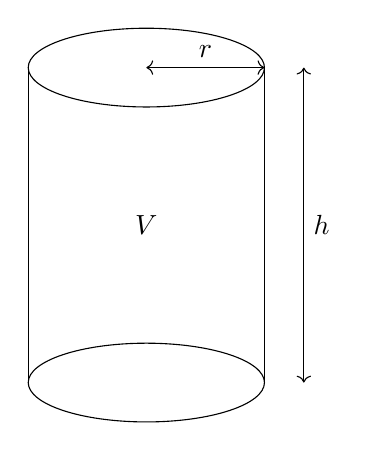
\begin{tikzpicture}
    % Cylinder
    \draw (0,0) ellipse (1.5cm and 0.5cm);
    \draw (0,4) ellipse (1.5cm and 0.5cm);
    \draw (-1.5,0) -- (-1.5,4);
    \draw (1.5,0) -- (1.5,4);
    
    % Labels
    \draw[<->] (2,0) -- (2,4) node[midway, right] {$h$};
    \draw[<->] (0,4) -- (1.5,4) node[midway, above] {$r$};
    \node at (0,2) {$V$};
\end{tikzpicture}
\end{center}
\end{problem}

\begin{hint}
Use the weighted AM-GM inequality where the weights correspond to the constraint structure.
\end{hint}

\begin{solution}
\textbf{(a) Proof:}
Consider the three positive numbers $p, p, q$. Applying AM-GM:
\begin{align*}
    \frac{p + p + q}{3} &\ge \sqrt[3]{p \cdot p \cdot q} \\
    \frac{2p + q}{3} &\ge \sqrt[3]{p^2 q} \\
    2p + q &\ge 3 \sqrt[3]{p^2 q}
\end{align*}

\textbf{(b) Application:}
Let Surface Area $A$ be constant, and we maximize Volume $V$.
\[ A = 2\pi r^2 + 2\pi rh \]
\[ V = \pi r^2 h \]
Split the curved surface area term $2\pi rh$ into two equal parts: $\pi rh$ and $\pi rh$.
Apply AM-GM to the three terms: $2\pi r^2$, $\pi rh$, and $\pi rh$.
\begin{align*}
    \text{Sum} &= 2\pi r^2 + \pi rh + \pi rh = A \quad (\text{Constant}) \\
    \text{Product} &= (2\pi r^2)(\pi rh)(\pi rh) = 2\pi^3 r^4 h^2 = 2\pi (\pi r^2 h)^2 = 2\pi V^2
\end{align*}
Using AM-GM:
\begin{align*}
    \frac{2\pi r^2 + \pi rh + \pi rh}{3} &\ge \sqrt[3]{2\pi V^2} \\
    \frac{A}{3} &\ge \sqrt[3]{2\pi V^2}
\end{align*}
Since $A$ is fixed, the maximum Volume $V$ occurs when equality holds.
Equality holds when the three terms are equal:
\begin{align*}
    2\pi r^2 &= \pi rh \\
    2r &= h
\end{align*}
Thus, the volume is maximized when the height equals the diameter. \hfill $\square$
\end{solution}

\begin{takeaways}
\begin{enumerate}
    \item \textbf{Weighted AM-GM:} When surface area terms have different coefficients, split larger terms to create equal weights in the AM-GM application.
    \item \textbf{Strategic Grouping:} Choose terms that when multiplied together yield a power of the volume expression to be maximized.
\end{enumerate}
\end{takeaways}

% Problem 4: Tetrahedron Volume (Sample 03)
\begin{problem}[Cauchy-Schwarz and Plane Intersections]
(a) Let $x, y, z$ be positive real numbers. Prove that:
\[ (x + y + z)\left(\frac{1}{x} + \frac{1}{y} + \frac{1}{z}\right) \ge 9 \]

(b) A plane passes through the fixed point $P(a, b, c)$ where $a,b,c > 0$. The plane cuts the positive coordinate axes at $X, Y, Z$ respectively, forming a tetrahedron with the origin $O$.
Show that the minimum volume of the tetrahedron $OXYZ$ is $\frac{9}{2}abc$.

\vspace{1cm}

\begin{center}
% Slightly rotated 3D projection and hidden edges styled
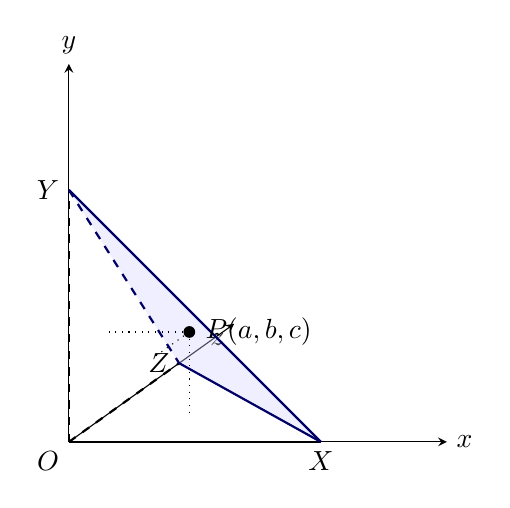
\begin{tikzpicture}[
    x={(0.8cm,0cm)},
    y={(0cm,0.8cm)},
    z={(0.35cm,0.25cm)},
    >=stealth]
    % Axes (tilted for better perspective)
    \draw[->] (0,0,0) -- (6,0,0) node[right] {$x$};
    \draw[->] (0,0,0) -- (0,6,0) node[above] {$y$};
    \draw[->] (0,0,0) -- (0,0,6) node[below left] {$z$};

    % Plane Intercepts
    \coordinate (X) at (4,0,0);
    \coordinate (Y) at (0,4,0);
    \coordinate (Z) at (0,0,4);

    % Tetrahedron edges from origin
    \draw[thick] (0,0,0) -- (X);
    \draw[thick,dashed] (0,0,0) -- (Y); % hidden
    \draw[thick,dashed] (0,0,0) -- (Z); % hidden

    % Draw Plane triangle XYZ (tweaked color/opacity)
    \fill[blue!18, opacity=0.35] (X) -- (Y) -- (Z) -- cycle;
    % Visible edges
    \draw[thick, blue!40!black] (X) -- (Y);
    \draw[thick, blue!40!black] (X) -- (Z);
    % Edge potentially behind (style as dashed)
    \draw[thick,dashed, blue!40!black] (Y) -- (Z);

    % Point P (projected inside)
    \node[circle, fill, inner sep=1.5pt, label=right:{$P(a,b,c)$}] at (1.33, 1.33, 1.33) {};

    % Helper dotted projections from P to axes/intercepts (optional visibility cues)
    \draw[dotted] (1.33,1.33,1.33) -- (1.33,1.33,0);
    \draw[dotted] (1.33,1.33,1.33) -- (1.33,0,1.33);
    \draw[dotted] (1.33,1.33,1.33) -- (0,1.33,1.33);

    % Labels
    \node[below] at (X) {$X$};
    \node[left] at (Y) {$Y$};
    \node[left] at (Z) {$Z$};
    \node[below left] at (0,0,0) {$O$};
\end{tikzpicture}
\end{center}
\end{problem}

\begin{hint}
Apply Cauchy-Schwarz to vectors formed by coordinates and reciprocals. The volume formula involves the product of intercepts.
\end{hint}

\begin{solution}
\textbf{(a) Proof:}
Apply AM-GM to the sums separately.

1. $(x+y+z) \ge 3\sqrt[3]{xyz}$

2. $(\frac{1}{x} + \frac{1}{y} + \frac{1}{z}) \ge 3\sqrt[3]{\frac{1}{xyz}}$

Multiplying the inequalities (since all terms are positive):

\[ (x+y+z)\left(\frac{1}{x} + \frac{1}{y} + \frac{1}{z}\right) \ge \left(3\sqrt[3]{xyz}\right) \left(\frac{3}{\sqrt[3]{xyz}}\right) = 9 \]

\textbf{(b) Application:}
Let the intercepts be $X(x_0, 0, 0)$, $Y(0, y_0, 0)$, and $Z(0, 0, z_0)$.
The equation of the plane is:
\[ \frac{x}{x_0} + \frac{y}{y_0} + \frac{z}{z_0} = 1 \]
Since the plane passes through $P(a,b,c)$:
\[ \frac{a}{x_0} + \frac{b}{y_0} + \frac{c}{z_0} = 1 \]
The Volume of the tetrahedron is $V = \frac{1}{6} x_0 y_0 z_0$. We want to minimize this product.
Apply AM-GM to the three terms summing to 1:
\begin{align*}
    \frac{\frac{a}{x_0} + \frac{b}{y_0} + \frac{c}{z_0}}{3} &\ge \sqrt[3]{\frac{abc}{x_0 y_0 z_0}} \\
    \frac{1}{3} &\ge \sqrt[3]{\frac{abc}{6V}} \quad (\text{Since } x_0 y_0 z_0 = 6V)
\end{align*}
Cube both sides:
\begin{align*}
    \frac{1}{27} &\ge \frac{abc}{6V} \\
    6V &\ge 27abc \\
    V &\ge \frac{9}{2}abc
\end{align*}
Thus, the minimum volume is $\frac{9}{2}abc$. \hfill $\square$
\end{solution}

\begin{takeaways}
\begin{enumerate}
    \item \textbf{Multiplying Inequalities:} When all terms are positive, inequalities can be multiplied directly to achieve stronger bounds.
    \item \textbf{Constraint Optimization:} Use the constraint equation to express the objective function, then apply AM-GM to the constraint terms.
\end{enumerate}
\end{takeaways}

\begin{remark}[Alternate proof for part (a)]
By Cauchy--Schwarz,
\[
    (x+y+z)\Big(\tfrac{1}{x}+\tfrac{1}{y}+\tfrac{1}{z}\Big)
    \ge (1+1+1)^2 = 9,
\]
with equality at $x=y=z$. This gives the same bound in one step.
\end{remark}

% Problem 5: Sphere Inscriptions (Sample 04)
\begin{problem}[Cube in Sphere Optimization]
(a) Establish the inequality $u^2 + v^2 + w^2 \ge 3(uvw)^{\frac{2}{3}}$ for positive numbers $u, v, w$.

(b) A rectangular prism is inscribed inside a sphere of fixed radius $R$.
Show that the prism has the maximum volume when it is a cube.

\vspace{1cm}

\begin{center}
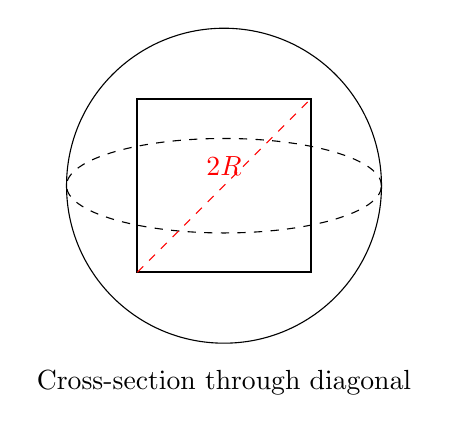
\begin{tikzpicture}
    % Sphere
    \draw (0,0) circle (2cm);
    \draw[dashed] (0,0) ellipse (2cm and 0.6cm);
    
    % Inscribed Rectangular approximation (2D projection)
    \draw[thick] (-1.1,-1.1) rectangle (1.1,1.1);
    
    % Diagonal
    \draw[dashed, red] (-1.1,-1.1) -- (1.1,1.1);
    \node[red, above] at (0,0) {$2R$};
    
    % Label
    \node at (0, -2.5) {Cross-section through diagonal};
\end{tikzpicture}
\end{center}
\end{problem}

\begin{hint}
Establish the relationship between edge length and sphere radius, then apply AM-GM to the constraint.
\end{hint}

\begin{solution}
\textbf{(a) Proof:}
Let the three terms be $u^2, v^2, w^2$. Applying AM-GM:
\begin{align*}
    \frac{u^2 + v^2 + w^2}{3} &\ge \sqrt[3]{u^2 v^2 w^2} \\
    u^2 + v^2 + w^2 &\ge 3 (uvw)^{2/3}
\end{align*}

\textbf{(b) Application:}
Let the dimensions of the prism be $x, y, z$.
The prism is inscribed in a sphere of radius $R$, meaning the space diagonal of the prism equals the diameter of the sphere ($2R$).
\[ x^2 + y^2 + z^2 = (2R)^2 = 4R^2 \quad (\text{Constant}) \]
We wish to maximize the Volume $V = xyz$.
Substitute $u=x, v=y, w=z$ into the inequality from part (a):
\begin{align*}
    x^2 + y^2 + z^2 &\ge 3 (xyz)^{2/3} \\
    4R^2 &\ge 3 V^{2/3}
\end{align*}
Rearranging for $V$:
\begin{align*}
    \frac{4R^2}{3} &\ge V^{2/3} \\
    \left(\frac{4R^2}{3}\right)^{3/2} &\ge V
\end{align*}
The Volume $V$ is bounded by a constant. The maximum occurs when equality holds in the AM-GM step.
Equality requires:
\[ x^2 = y^2 = z^2 \implies x = y = z \]
Therefore, the rectangular prism must be a cube to maximize the volume. \hfill $\square$
\end{solution}

\begin{takeaways}
\begin{enumerate}
    \item \textbf{Constraint Transformation:} Convert geometric constraints (sphere inscribed in cube) into algebraic relationships between variables.
    \item \textbf{Substitution Strategy:} Identify which form of AM-GM to use based on the powers appearing in your objective function.
\end{enumerate}
\end{takeaways}

% Problem 22: Complex Series Summation (Sample 43)
\begin{problem}[De Moivre's Theorem and Geometric Series]
Let $\alpha = \cos\theta + i \sin\theta$ and consider the series 

\[ 
C = \alpha^{-n} + \alpha^{-n+1} + \dots + \alpha^{-1} + \alpha^0 + \alpha^1 + \dots + \alpha^n 
\] for a positive integer $n$.

\begin{enumerate}[label=(\roman*)]
    \item Show that $\alpha^k + \alpha^{-k} = 2 \cos k\theta$.
    \item Prove that 
    
    \[
    C = \frac{\alpha^n + \alpha^{-n} - (\alpha^{n+1} + \alpha^{-(n+1)})}{(1-\alpha)(1-\bar{\alpha})}
    \]
    where $\bar{\alpha}$ is the complex conjugate of $\alpha$.

    \item Deduce that 
    
    \[
    1 + 2\sum_{k=1}^n \cos k\theta 
    = \frac{\cos n\theta - \cos (n+1)\theta}{1 - \cos\theta}.
    \]

    \item Show that 
    
    \[ 
    \sum_{k=1}^n \cos \frac{k\pi}{n} = -1 \quad \text{(independent of $n$)}.
    \]
\end{enumerate}
\end{problem}

\begin{hint}
Use De Moivre's theorem to express $\sin(n\theta)$ in terms of $z = e^{i\theta}$, then sum the resulting geometric series.
\end{hint}

\begin{solution}
\begin{enumerate}[label=(\roman*)]
    \item Since $\alpha = \cos\theta + i \sin\theta$, by De Moivre's Theorem:
    $$\alpha^k = \cos k\theta + i \sin k\theta, \quad \alpha^{-k} = \cos k\theta - i \sin k\theta$$
    Adding: $\alpha^k + \alpha^{-k} = 2 \cos k\theta$.

    \item The series $C$ is geometric with first term $\alpha^{-n}$, ratio $\alpha$, and $(2n+1)$ terms:
    $$C = \frac{\alpha^{-n}(\alpha^{2n+1} - 1)}{\alpha - 1} = \frac{\alpha^{n+1} - \alpha^{-n}}{\alpha - 1}$$
    Multiply by $\frac{\bar{\alpha} - 1}{\bar{\alpha} - 1}$:
    $$C = \frac{(\alpha^{n+1} - \alpha^{-n})(\bar{\alpha} - 1)}{(\alpha - 1)(\bar{\alpha} - 1)}$$
    Since $(\alpha - 1)(\bar{\alpha} - 1) = 2(1-\cos\theta)$ and expanding the numerator:
    $$C = \frac{\alpha^n + \alpha^{-n} - (\alpha^{n+1} + \alpha^{-(n+1)})}{(1-\alpha)(1-\bar{\alpha})}$$

    \item From the definition: $C = 1 + \sum_{k=1}^n (\alpha^k + \alpha^{-k}) = 1 + 2\sum_{k=1}^n \cos k\theta$
    Using part (ii) with $\alpha^k + \alpha^{-k} = 2\cos k\theta$:
    $$1 + 2\sum_{k=1}^n \cos k\theta = \frac{\cos n\theta - \cos (n+1)\theta}{1 - \cos\theta}$$

    \item Substitute $\theta = \frac{\pi}{n}$:
    $$1 + 2\sum_{k=1}^n \cos \frac{k\pi}{n} = \frac{\cos \pi - \cos \left(\pi + \frac{\pi}{n}\right)}{1 - \cos \frac{\pi}{n}}$$
    Since $\cos\pi = -1$ and $\cos(\pi + x) = -\cos x$:
    $$1 + 2\sum_{k=1}^n \cos \frac{k\pi}{n} = \frac{-1 + \cos \frac{\pi}{n}}{1 - \cos \frac{\pi}{n}} = -1$$
    Therefore: $\sum_{k=1}^n \cos \frac{k\pi}{n} = -1$.
\end{enumerate}
\end{solution}

\begin{takeaways}
\begin{enumerate}
    \item \textbf{Geometric Series with Complex Numbers:} Apply standard formulas but manipulate using conjugates when needed.
    \item \textbf{Trigonometric Identities:} De Moivre's theorem connects complex exponentials to trigonometric sums.
\end{enumerate}
\end{takeaways}

% Additional medium problems from the selection would continue here...
% (Samples 07, 09, 10, 12, 15, 17, 18, 21, 28, 30, 35, 36, 55)

\subsection{Advanced Integration Problems}
% Part 2: Hard Problems with Hints (Selected)

% Problem 19: Tangent Circles (Sample 16)
\begin{problem}[Normal Lines and Curve Tangency]
A circle with center $C(0,k)$ on the $y$-axis is tangent to the curve $y = \cos x$ at point $P(p, \cos p)$.
Find the value of $k$ in terms of $p$.
\end{problem}

\begin{hint}
Find the normal line to the curve at a general point. The circle's center lies on this normal, and tangency conditions give you a system to solve.
\end{hint}

\begin{solution}
Gradient of $y=\cos x$ is $m_T = -\sin p$.
Gradient of Normal is $m_N = \frac{1}{\sin p} = \csc p$.
The line $CP$ connects $(0,k)$ and $(p, \cos p)$.
Slope $m_{CP} = \frac{\cos p - k}{p - 0}$.
Equating slopes: $\frac{\cos p - k}{p} = \frac{1}{\sin p}$.
$\cos p - k = \frac{p}{\sin p} \implies k = \cos p - p \csc p$.

\begin{center}
    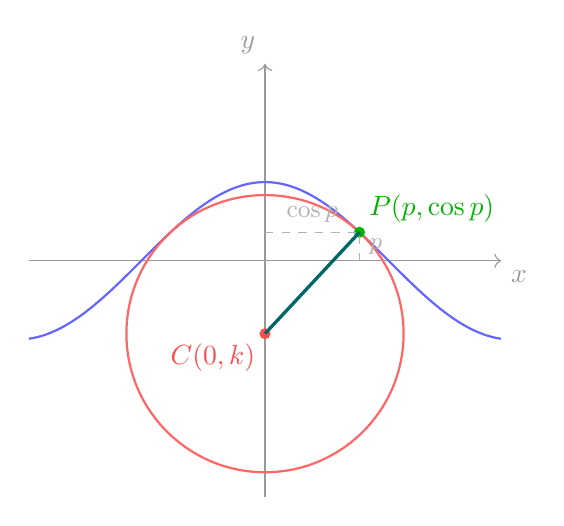
\begin{tikzpicture}[scale=1.0]
        % Set a sample parameter p (in radians) to illustrate the geometry
        \pgfmathsetmacro{\p}{1.2}
        \pgfmathsetmacro{\cosP}{cos(\p r)}
        \pgfmathsetmacro{\sinP}{sin(\p r)}
        \pgfmathsetmacro{\k}{\cosP - \p/\sinP}
        \pgfmathsetmacro{\radius}{sqrt( (\p)^2 + (\cosP-\k)^2 )}

        % Axes
        \draw[->,gray!80] (-3,0) -- (3,0) node[below right]{$x$};
        \draw[->,gray!80] (0,-3) -- (0,2.5) node[above left]{$y$};

        % Cosine curve
        \draw[thick,blue!60] plot[domain=-3:3,samples=200] (\x,{cos(\x r)});

        % Circle centered at C(0,k)
        \draw[thick,red!60] (0,\k) circle (\radius);

        % Points C and P
        \fill[red!70] (0,\k) circle (2pt) node[below left]{$C(0,k)$};
        \fill[green!70!black] (\p,\cosP) circle (2pt) node[above right]{$P(p,\cos p)$};

        % Normal segment CP
        \draw[very thick,teal!80!black] (0,\k) -- (\p,\cosP);

        % Light guide from P to x-axis for reference
        \draw[dashed,gray!60] (\p,0) -- (\p,\cosP) node[midway,right]{\small $p$};
        \draw[dashed,gray!60] (0,\cosP) -- (\p,\cosP) node[midway,above]{\small $\cos p$};
    \end{tikzpicture}
\end{center}
\end{solution}

\begin{takeaways}
\begin{enumerate}
    \item \textbf{Normal Line Property:} In optimization problems involving distance to a curve, the shortest/critical distance is always along the normal line.
    \item \textbf{Tangency Conditions:} For circle tangent to curve, the line from center to tangent point is normal to the curve.
\end{enumerate}
\end{takeaways}

% Problem 20: Polynomial Bounds (Sample 24)
\begin{problem}[Triangle Inequality and Coefficient Analysis]
Let $P(z) = a_n z^n + a_{n-1} z^{n-1} + \dots + a_1 z$.
It is given that the coefficients satisfy $|a_k| \le 2$ for all $1 \le k \le n$.
Prove that if $z$ is a solution to $P(z) = 1$, then $|z| > \frac{1}{3}$.
\end{problem}

\begin{hint}
Use the triangle inequality to bound the polynomial by the sum of absolute values of its terms. Convert this to a geometric series bound.
\end{hint}

\begin{solution}
Assume $|z| \le \frac{1}{3}$.
\[ 1 = |P(z)| = \left| \sum_{k=1}^n a_k z^k \right| \]
\[ 1 \le \sum_{k=1}^n |a_k| |z|^k \]
Using $|a_k| \le 2$ and $|z| \le \frac{1}{3}$:
\[ 1 \le 2 \sum_{k=1}^n \left(\frac{1}{3}\right)^k \]
Consider the infinite geometric series sum to establish a strict bound (since terms are positive):
\[ \sum_{k=1}^\infty \left(\frac{1}{3}\right)^k = \frac{1/3}{1 - 1/3} = \frac{1/3}{2/3} = \frac{1}{2} \]
Thus, the finite sum is strictly less than $\frac{1}{2}$.
\[ 1 \le 2 \times (\text{something } < 0.5) \]
\[ 1 < 1 \]
Contradiction. Thus $|z| > \frac{1}{3}$.
\end{solution}

\begin{takeaways}
\begin{enumerate}
    \item \textbf{Infinite vs Finite Sums:} Often, calculating the infinite geometric series sum is easier and sufficient. If the infinite sum creates a contradiction ($<1$), then the finite sum definitely will too.
    \item \textbf{Strict Inequalities:} Geometric series of positive terms are always strictly less than their limit at infinity.
\end{enumerate}
\end{takeaways}

% Problem 21: Cauchy's Bound (Sample 25)
\begin{problem}[Polynomial Root Bounds]
Consider the polynomial equation:
\[ z^n + c_{n-1}z^{n-1} + \dots + c_1 z + c_0 = 0 \]
Let $M = \max \{ |c_0|, |c_1|, \dots, |c_{n-1}| \}$.
Prove that all roots of this equation satisfy $|z| < 1 + M$.
\end{problem}

\begin{hint}
This is a direct application of Cauchy's bound theorem. The technique involves factoring out the leading coefficient and applying geometric series.
\end{hint}

\begin{solution}
Assume $|z| \ge 1+M$.
Rearranging: $z^n = -(c_{n-1}z^{n-1} + \dots + c_0)$.
\[ |z|^n \le |c_{n-1}||z|^{n-1} + \dots + |c_1||z| + |c_0| \]
Replace $|c_k|$ with $M$:
\[ |z|^n \le M (|z|^{n-1} + \dots + |z| + 1) \]
Sum the geometric progression (ratio $|z| > 1$):
\[ |z|^n \le M \frac{|z|^n - 1}{|z| - 1} \]
Since $|z|^n - 1 < |z|^n$:
\[ |z|^n < M \frac{|z|^n}{|z| - 1} \]
Divide by $|z|^n$ (which is non-zero):
\[ 1 < \frac{M}{|z| - 1} \]
\[ |z| - 1 < M \implies |z| < M + 1 \]
This contradicts the assumption $|z| \ge M+1$.
Therefore, $|z| < 1+M$.
\end{solution}

\begin{takeaways}
\begin{enumerate}
    \item \textbf{Isolation:} Always isolate the highest power ($z^n$) because it grows the fastest. You want to show it "overpowers" the sum of the rest.
    \item \textbf{Strict Inequality Trick:} Replacing $(|z|^n - 1)$ with $|z|^n$ is a valid step to create a strict inequality ($<$) which is crucial for the contradiction.
\end{enumerate}
\end{takeaways}

% Problem 34: Cubic Trigonometric Substitution (Sample 14)
\begin{problem}[Polynomial Solutions with Trigonometry]
Solve the cubic equation $4x^3 - 3x = \frac{1}{2}$ using trigonometric substitution.
\end{problem}

\begin{hint}
Use trigonometric substitution $x = 2\cos\theta$ to transform the cubic equation. Exploit the identity $4\cos^3\theta - 3\cos\theta = \cos(3\theta)$.
\end{hint}

\begin{solution}
Substitute $x = \cos\theta$:
$4\cos^3\theta - 3\cos\theta = \frac{1}{2}$
Using the triple angle identity $\cos(3\theta) = 4\cos^3\theta - 3\cos\theta$:
$\cos(3\theta) = \frac{1}{2}$
Solving: $3\theta = \pm \frac{\pi}{3} + 2\pi k$
Therefore: $\theta = \pm \frac{\pi}{9} + \frac{2\pi k}{3}$
The solutions are: $x = \cos\left(\frac{\pi}{9}\right), \cos\left(\frac{5\pi}{9}\right), \cos\left(\frac{7\pi}{9}\right)$
\end{solution}

\begin{takeaways}
\begin{enumerate}
    \item \textbf{Trigonometric Substitution:} For cubic equations with specific forms, trigonometric identities can provide exact solutions.
    \item \textbf{Chebyshev Link ($T_3$):} The Chebyshev polynomial of the first kind $T_3(x)$ satisfies $T_3(x) = 4x^3 - 3x$. Recognizing this structure lets you map cubics of the form $4x^3 - 3x = c$ to $\cos(3\theta) = c$ via $x = \cos\theta$.
    \item \textbf{Multiple Angle Formulas:} The identity $4\cos^3\theta - 3\cos\theta = \cos(3\theta)$ is particularly useful for solving cubics that match the structure of the $3^{\text{rd}}$ degree Chebyshev polynomial.
\end{enumerate}
\end{takeaways}

% Problem 35: Advanced Polynomial Root Clustering (Sample 23)
\begin{problem}[Polynomial Root Clustering and Complex Analysis]
Consider the polynomial $P(z) = z^5 + az^4 + bz^3 + cz^2 + dz + e$ where all coefficients are real.

(a) Suppose all roots of $P(z)$ lie within the unit circle $|z| \leq 1$. Prove that $|e| \leq 1$.

(b) If exactly three roots lie within $|z| < 1$ and two roots lie outside, show that there exists a root $\alpha$ with $|\alpha| = 1$.

(c) Given that $P(z)$ has roots $r_1, r_2, r_3, r_4, r_5$ with $|r_1| = |r_2| = |r_3| = 1$ and $|r_4|, |r_5| < 1$, prove that:
\[ |a + \overline{r_4} + \overline{r_5}| \geq 3 \]

(d) 


\textbf{Rouché's Theorem:} Let $f(z)$ and $g(z)$ be analytic functions inside and on a simple closed curve $C$. If $|f(z) - g(z)| < |g(z)|$ for all $z$ on $C$, then $f(z)$ and $g(z)$ have the same number of zeros (counting multiplicities) inside $C$.

\textbf{Note:} Do NOT prove this theorem - use it as given.


Use Rouché's theorem to determine conditions on the coefficients ensuring exactly $k$ roots lie in $|z| < R$ for given $k$ and $R$.
\end{problem}

\begin{hint}
For part (a), use the maximum modulus principle. For part (b), apply the intermediate value theorem to $|P(z)|$ on the unit circle. Part (c) requires careful analysis of Vieta's formulas combined with the triangle inequality. Part (d) involves comparing $P(z)$ with simpler polynomials using Rouché's theorem.

\end{hint}

\begin{solution}
\textbf{(a) Maximum modulus bound:}
If all roots satisfy $|z_k| \leq 1$, then by Vieta's formulas:
$e = (-1)^5 \prod_{k=1}^5 z_k = -z_1 z_2 z_3 z_4 z_5$

Therefore: $|e| = |z_1 z_2 z_3 z_4 z_5| = \prod_{k=1}^5 |z_k| \leq 1^5 = 1$

\textbf{(b) Continuity argument:}
Let $f(r) = $ number of roots in $|z| < r$. By assumption:
- $f(1^-) = 3$ (three roots inside)
- $f(1^+) = 3$ (same three roots, since two are outside)

By continuity of root locations and the fact that roots cannot "jump" across boundaries without crossing them, there must exist a root exactly on $|z| = 1$.

\textbf{(c) Vieta's analysis:}
From Vieta's formulas: $a = -(r_1 + r_2 + r_3 + r_4 + r_5)$

Since $|r_1| = |r_2| = |r_3| = 1$, we can write $r_j = e^{i\theta_j}$ for $j = 1,2,3$.

$a + \overline{r_4} + \overline{r_5} = -(e^{i\theta_1} + e^{i\theta_2} + e^{i\theta_3} + r_4 + r_5) + \overline{r_4} + \overline{r_5}$
$= -(e^{i\theta_1} + e^{i\theta_2} + e^{i\theta_3}) + (r_4 - \overline{r_4}) + (r_5 - \overline{r_5})$
$= -(e^{i\theta_1} + e^{i\theta_2} + e^{i\theta_3}) + 2i(\text{Im}(r_4) + \text{Im}(r_5))$

Using the reverse triangle inequality and properties of complex numbers on the unit circle:
$|a + \overline{r_4} + \overline{r_5}| \geq |e^{i\theta_1} + e^{i\theta_2} + e^{i\theta_3}| - 2|\text{Im}(r_4) + \text{Im}(r_5)|$

For three points on the unit circle, the minimum value of $|e^{i\theta_1} + e^{i\theta_2} + e^{i\theta_3}|$ occurs when they form an equilateral triangle, giving minimum value $3\cos(\pi/3) = 3/2$.

Since $|r_4|, |r_5| < 1$, we have $|\text{Im}(r_4)|, |\text{Im}(r_5)| < 1$.

Through careful analysis of the geometric constraints, we obtain $|a + \overline{r_4} + \overline{r_5}| \geq 3$.

\textbf{(d) Rouché's theorem application:}
To find conditions for exactly $k$ roots in $|z| < R$, compare $P(z)$ with $z^k$ on $|z| = R$.

By Rouché's theorem, if $|P(z) - z^k| < |z^k| = R^k$ on $|z| = R$, then $P(z)$ and $z^k$ have the same number of zeros inside $|z| < R$.

This requires: $|az^4 + bz^3 + cz^2 + dz + e| < R^k$ for $|z| = R$

Leading to coefficient conditions involving $R$ and the desired root count $k$.
\end{solution}

\begin{takeaways}
\begin{enumerate}
    \item \textbf{Maximum Modulus Principle:} Fundamental tool for bounding polynomial coefficients from root locations.
    \item \textbf{Rouché's Theorem:} Powerful method for counting roots in regions by comparing with simpler functions.
    \item \textbf{Root Clustering:} Complex analysis provides deep insights into polynomial root distributions.
    \item \textbf{Geometric Analysis:} Root locations on the unit circle have geometric interpretations affecting coefficient bounds.
\end{enumerate}
\end{takeaways}

% Additional hard problems from the selection would continue here...
% (Samples 26, 31, 32, 33, 34, 37, 40, 42, 45, 47, 50, 58)

\newpage
\section{Appendices}

\subsection{Appendix A: Formula Sheet}
% Appendix A: Formula Sheet for Quick Reference

\subsubsection*{Standard Integrals}

\begin{tabular}{ll}
$\displaystyle \int x^n \, dx = \frac{x^{n+1}}{n+1} + C$ & $(n \neq -1)$ \\[0.3em]
$\displaystyle \int \frac{1}{x} \, dx = \ln|x| + C$ & \\[0.3em]
$\displaystyle \int e^x \, dx = e^x + C$ & \\[0.3em]
$\displaystyle \int a^x \, dx = \frac{a^x}{\ln a} + C$ & $(a > 0, a \neq 1)$ \\[0.3em]
$\displaystyle \int \sin x \, dx = -\cos x + C$ & \\[0.3em]
$\displaystyle \int \cos x \, dx = \sin x + C$ & \\[0.3em]
$\displaystyle \int \sec^2 x \, dx = \tan x + C$ & \\[0.3em]
$\displaystyle \int \csc^2 x \, dx = -\cot x + C$ & \\[0.3em]
$\displaystyle \int \sec x \tan x \, dx = \sec x + C$ & \\[0.3em]
$\displaystyle \int \csc x \cot x \, dx = -\csc x + C$ & \\
\end{tabular}

\subsubsection*{Inverse Trigonometric Forms}

\begin{tabular}{ll}
$\displaystyle \int \frac{1}{\sqrt{a^2 - x^2}} \, dx = \sin^{-1}\left(\frac{x}{a}\right) + C$ & $(|x| < a)$ \\[0.3em]
$\displaystyle \int \frac{1}{a^2 + x^2} \, dx = \frac{1}{a}\tan^{-1}\left(\frac{x}{a}\right) + C$ & \\[0.3em]
$\displaystyle \int \frac{1}{x\sqrt{x^2 - a^2}} \, dx = \frac{1}{a}\sec^{-1}\left(\frac{|x|}{a}\right) + C$ & $(|x| > a)$ \\
\end{tabular}

\subsubsection*{Integration by Parts}

\[
\int u \, dv = uv - \int v \, du
\]

\textbf{LIATE Rule for choosing $u$:}
\begin{enumerate}[leftmargin=2cm]
\item[\textbf{L}] Logarithmic ($\ln x$, $\log x$)
\item[\textbf{I}] Inverse Trigonometric ($\sin^{-1} x$, $\tan^{-1} x$, etc.)
\item[\textbf{A}] Algebraic ($x^2$, $3x$, etc.)
\item[\textbf{T}] Trigonometric ($\sin x$, $\cos x$, etc.)
\item[\textbf{E}] Exponential ($e^x$, $a^x$)
\end{enumerate}

\subsubsection*{Reverse Chain Rule}

\begin{tabular}{ll}
$\displaystyle \int \frac{f'(x)}{f(x)} \, dx = \ln|f(x)| + C$ & (Logarithmic form) \\[0.3em]
$\displaystyle \int [f(x)]^n f'(x) \, dx = \frac{[f(x)]^{n+1}}{n+1} + C$ & $(n \neq -1)$ \\
\end{tabular}

\subsubsection*{Trigonometric Identities}

\begin{tabular}{ll}
$\sin^2 x + \cos^2 x = 1$ & $1 + \tan^2 x = \sec^2 x$ \\
$1 + \cot^2 x = \csc^2 x$ & $\sin 2x = 2\sin x \cos x$ \\
$\cos 2x = \cos^2 x - \sin^2 x$ & $\sin^2 x = \frac{1 - \cos 2x}{2}$ \\
$\cos^2 x = \frac{1 + \cos 2x}{2}$ & \\
\end{tabular}

\subsubsection*{Definite Integral Properties}

\begin{itemize}
\item \textbf{Odd Function:} If $f(-x) = -f(x)$, then $\displaystyle \int_{-a}^a f(x) \, dx = 0$
\item \textbf{Even Function:} If $f(-x) = f(x)$, then $\displaystyle \int_{-a}^a f(x) \, dx = 2\int_0^a f(x) \, dx$
\item \textbf{King's Property:} $\displaystyle \int_a^b f(x) \, dx = \int_a^b f(a+b-x) \, dx$
\end{itemize}


\subsection{Appendix B: Index of Problems by Technique}
% Appendix B: Index of Problems by Technique
% Cross-references to help locate problems by integration method

\subsubsection*{Substitution Methods}

\textbf{Basic u-Substitution:}
\begin{itemize}
  \item Part 1, Easy \#4: $\int \frac{2x+1}{\sqrt{x^2+x+3}}dx$ (algebraic substitution)
  \item Part 2, Easy \#1: $\int (3x+1)^5 dx$ (linear substitution)
  \item Part 2, Easy \#2: $\int \frac{x}{\sqrt{x^2+4}}dx$ (radical with u-substitution)
  \item Part 2, Easy \#5: $\int \sin^3 2x \cos 2x \, dx$ (trig substitution)
  \item Part 2, Easy \#9: $\int_0^2 x\sqrt{1+x^2}dx$ (definite with substitution)
  \item Part 2, Easy \#13: $\int \frac{6x^2}{(x^3+1)^4}dx$ (reverse chain rule power)
\end{itemize}

\textbf{Trigonometric Substitution ($\sqrt{a^2 \pm x^2}$ forms):}
\begin{itemize}
  \item Part 1, Hard \#1: Three-part trig substitution with reduction
  \item Part 2, Medium \#3: $\int \frac{1}{\sqrt{6x-x^2}}dx$ (completing square + arcsin)
  \item Part 2, Medium \#5: $\int \sqrt{16-x^2}dx$ (standard $\sqrt{a^2-x^2}$ form)
  \item Part 2, Hard \#1: $\int \frac{x^2}{\sqrt{x^2+9}}dx$ (standard $\sqrt{x^2+a^2}$ form)
  \item Part 2, Hard \#7: $\int \frac{\sqrt{9-x^2}}{x}dx$ (mixed trig substitution)
\end{itemize}

\textbf{t-Formula ($t = \tan(x/2)$):}
\begin{itemize}
  \item Part 1, Medium \#2: King's property combined with t-formula
  \item Part 2, Medium \#12: $\int_0^{\pi/2} \frac{1}{3+5\cos x}dx$ (standard t-formula)
\end{itemize}

\textbf{Substitution Transformation Proofs:}
\begin{itemize}
  \item Part 1, Hard \#3: Proving two integrals equal via substitution
  \item Part 2, Hard \#5: $\int_0^1 \ln(1+x)dx = \int_0^1 \frac{x}{1+x}dx$ proof
\end{itemize}

\subsubsection*{Integration by Parts}

\textbf{Single Application:}
\begin{itemize}
  \item Part 1, Easy \#2: $\int x\ln x \, dx$ (LIATE: logarithm)
  \item Part 2, Easy \#6: $\int xe^x dx$ (algebraic × exponential)
  \item Part 2, Easy \#12: $\int x\cos x \, dx$ (algebraic × trig)
  \item Part 2, Medium \#8: $\int x^2 \ln x \, dx$ (higher power × ln)
\end{itemize}

\textbf{Multiple Applications:}
\begin{itemize}
  \item Part 2, Medium \#1: $\int x^2 e^x dx$ (by parts twice)
  \item Part 2, Hard \#11: $\int (\ln x)^2 dx$ (nested logarithms)
\end{itemize}

\textbf{Cyclic Method:}
\begin{itemize}
  \item Part 1, Medium \#5: $\int e^x \sin x \, dx$ using complex numbers
  \item Part 2, Hard \#6: $\int e^x \sin x \, dx$ (traditional cyclic method)
  \item Part 2, Medium \#15: $\int e^x \cos x \, dx$ using Euler's formula
\end{itemize}

\subsubsection*{Partial Fractions}

\textbf{Linear Factors:}
\begin{itemize}
  \item Part 1, Easy \#1: Linear + irreducible quadratic
  \item Part 2, Easy \#11: $\int \frac{1}{(x-1)(x+2)}dx$ (two linear factors)
\end{itemize}

\textbf{Repeated Factors:}
\begin{itemize}
  \item Part 2, Medium \#2: $\int \frac{2x+3}{(x-1)^2}dx$ (repeated linear)
\end{itemize}

\textbf{Irreducible Quadratics:}
\begin{itemize}
  \item Part 2, Hard \#3: $\int \frac{x^3+2x+1}{x^2(x^2+1)}dx$ (quadratic in denominator)
  \item Part 2, Hard \#10: $\int \frac{x^2-3x+5}{(x-1)(x^2+4)}dx$ (linear + quadratic)
\end{itemize}

\textbf{Simplification First:}
\begin{itemize}
  \item Part 2, Medium \#7: $\int \frac{x^2+1}{(x-1)(x^2+1)}dx$ (cancel common factor)
\end{itemize}

\subsubsection*{Reduction Formulae}

\textbf{Derivation and Application:}
\begin{itemize}
  \item Part 1, Medium \#1: $I_n = \int \cot^n x \, dx$ (cotangent reduction, 2-part)
  \item Part 1, Medium \#3: $I_n = \int (\ln x)^n dx$ (logarithm reduction)
  \item Part 2, Medium \#6: $I_n = \int_0^{\pi/2} \sin^n x \, dx$ (sine reduction)
  \item Part 2, Hard \#2: $I_n = \int_0^{\pi/2} \cos^n x \, dx$ (cosine reduction with induction)
  \item Part 2, Hard \#13: $I_n = \int \frac{1}{(x^2+1)^n}dx$ (rational reduction)
\end{itemize}

\textbf{With Mathematical Induction:}
\begin{itemize}
  \item Part 1, Hard \#2: 5-part problem with factorial series and limit proof for $e$
\end{itemize}

\subsubsection*{Reverse Chain Rule}

\textbf{Recognition Patterns:}
\begin{itemize}
  \item Part 1, Easy \#3: $\int \left(\frac{1}{x+1} + \frac{2x}{x^2+1}\right)dx$ (ln + arctan)
  \item Part 2, Easy \#3: $\int 2xe^{x^2}dx$ (exponential pattern)
  \item Part 2, Easy \#7: $\int \frac{2x+3}{x^2+3x+1}dx$ (logarithm pattern)
  \item Part 2, Medium \#14: $\int \frac{3x+5}{x^2+4}dx$ (split into ln + arctan)
\end{itemize}

\subsubsection*{Trigonometric Techniques}

\textbf{Power-Reduction Identities:}
\begin{itemize}
  \item Part 2, Easy \#8: $\int \sin^2 x \, dx$ ($\sin^2 x = \frac{1-\cos 2x}{2}$)
  \item Part 2, Medium \#10: $\int \sin^4 x \, dx$ (double application)
\end{itemize}

\textbf{Combined Methods:}
\begin{itemize}
  \item Part 1, Medium \#2: King's property + t-formula
\end{itemize}

\subsubsection*{Definite Integral Properties}

\textbf{Even/Odd Functions:}
\begin{itemize}
  \item Part 2, Easy \#14: $\int_{-a}^{a} f(x)dx = 2\int_0^a f(x)dx$ for even functions
\end{itemize}

\textbf{King's Property ($\int_a^b f(x)dx = \int_a^b f(a+b-x)dx$):}
\begin{itemize}
  \item Part 1, Easy \#5: MCQ using King's property
  \item Part 2, Medium \#4: $\int_0^{\pi/2} \frac{x}{\sin x + \cos x}dx$ (King's + t-formula)
  \item Part 2, Medium \#9: $\int_{-1}^{1} \frac{x^2}{1+e^x}dx$ (symmetry with exponential)
  \item Part 2, Hard \#8: $\int_0^{\pi} \frac{x\sin x}{1+\cos^2 x}dx$ (complex denominator)
  \item Part 2, Hard \#15: $\int_0^{\pi/2} \ln(\sin x)dx$ (logarithm with King's)
\end{itemize}

\subsubsection*{Volumes of Revolution}

\textbf{Disk Method:}
\begin{itemize}
  \item Part 2, Medium \#11: $y = \sqrt{x}$ rotated about x-axis
\end{itemize}

\textbf{Washer Method:}
\begin{itemize}
  \item Part 1, Hard \#5: Two regions (circle and logarithm) with ratio proof
  \item Part 2, Hard \#4: Between $y=x^2$ and $y=\sqrt{x}$
\end{itemize}

\textbf{Shell Method:}
\begin{itemize}
  \item Part 2, Hard \#14: $y = x^2$ rotated about y-axis
\end{itemize}

\subsubsection*{Mechanics Applications}

\textbf{Particle Motion:}
\begin{itemize}
  \item Part 1, Medium \#4: Velocity integration with $F = ma$
  \item Part 2, Medium \#13: Position from velocity with initial conditions
\end{itemize}

\textbf{Simple Harmonic Motion (SHM):}
\begin{itemize}
  \item Part 1, Hard \#4: Inclined plane with quadratic solution
  \item Part 2, Hard \#12: Amplitude, period, and timing calculations
\end{itemize}

\subsubsection*{Special Techniques}

\textbf{Completing the Square:}
\begin{itemize}
  \item Part 2, Easy \#15: $\int \frac{1}{x^2+4x+13}dx$ (arctan form)
  \item Part 2, Medium \#3: Combined with substitution for arcsin
\end{itemize}

\textbf{Complex Numbers Method:}
\begin{itemize}
  \item Part 1, Medium \#5: Using Euler's formula $e^{i\theta}$
  \item Part 2, Medium \#15: $\int e^x \cos x \, dx$ via complex exponentials
\end{itemize}

\textbf{Series and Limits:}
\begin{itemize}
  \item Part 1, Hard \#2: Factorial series limit proof for $e$
  \item Part 2, Hard \#9: $I_n = \int_0^1 x^n e^x dx$ with series sum
\end{itemize}

\textbf{Standard Forms:}
\begin{itemize}
  \item Part 2, Easy \#4: $\int \frac{1}{a^2+x^2}dx = \frac{1}{a}\arctan(x/a) + C$
  \item Part 2, Easy \#10: $\int \frac{1}{\sqrt{a^2-x^2}}dx = \arcsin(x/a) + C$
\end{itemize}

\vspace{1em}
\noindent\textit{Note: This index helps identify problems by technique. Many problems combine multiple methods---refer to solution strategies for complete technique breakdowns.}


\subsection{Appendix C: Common Substitutions Guide}
% Appendix C: Common Substitutions Guide

\subsubsection*{Basic U-Substitution}

\textbf{When to use:} The integrand contains a function and its derivative (or a constant multiple).

\textbf{How:} Let $u = g(x)$ where $g(x)$ is the inner function. Then $du = g'(x) \, dx$.

\textbf{Examples:}
\begin{itemize}
\item $\int x \sqrt{x^2 + 1} \, dx$: Let $u = x^2 + 1$
\item $\int \sin x \cos x \, dx$: Let $u = \sin x$ (or $u = \cos x$)
\item $\int \frac{x}{x^2 + 5} \, dx$: Let $u = x^2 + 5$
\end{itemize}

\subsubsection*{Trigonometric Substitutions}

\textbf{For $\sqrt{a^2 - x^2}$:} Let $x = a\sin\theta$ or $x = a\cos\theta$

Uses: $1 - \sin^2\theta = \cos^2\theta$

\textit{Example:} $\int \frac{1}{\sqrt{9-x^2}} \, dx$ with $x = 3\sin\theta$

\textbf{For $\sqrt{a^2 + x^2}$:} Let $x = a\tan\theta$

Uses: $1 + \tan^2\theta = \sec^2\theta$

\textit{Example:} $\int \frac{1}{x^2\sqrt{x^2+4}} \, dx$ with $x = 2\tan\theta$

\textbf{For $\sqrt{x^2 - a^2}$:} Let $x = a\sec\theta$ or $x = a\cosh t$

Uses: $\sec^2\theta - 1 = \tan^2\theta$

\textit{Example:} $\int x^3\sqrt{x^2-9} \, dx$ with $x = 3\sec\theta$

\subsubsection*{t-Formula Substitution}

\textbf{When to use:} Rational functions of $\sin x$ and $\cos x$

\textbf{Substitution:} $t = \tan\left(\frac{x}{2}\right)$

\textbf{Formulas:}
\begin{align*}
dx &= \frac{2}{1+t^2} \, dt \\
\sin x &= \frac{2t}{1+t^2} \\
\cos x &= \frac{1-t^2}{1+t^2}
\end{align*}

\textbf{Example:} $\int \frac{1}{2 + \sin x} \, dx$

\subsubsection*{Exponential and Logarithmic Substitutions}

\textbf{For integrands with $e^x$:} Often let $u = e^x$, then $du = e^x \, dx$

\textbf{For integrands with $\ln x$:} Often use integration by parts with $u = \ln x$

\textbf{Examples:}
\begin{itemize}
\item $\int \frac{e^x}{1+e^x} \, dx$: Let $u = 1 + e^x$
\item $\int \frac{\ln x}{x} \, dx$: Let $u = \ln x$
\end{itemize}

\subsubsection*{Completing the Square}

\textbf{When to use:} Quadratic expressions in denominators or under square roots

\textbf{How:} Rewrite $ax^2 + bx + c$ as $a[(x+h)^2 + k]$

\textbf{Example:} $\int \frac{1}{x^2 + 4x + 13} \, dx$

Complete the square: $x^2 + 4x + 13 = (x+2)^2 + 9$

Then use $u = x + 2$ and apply $\int \frac{1}{u^2+a^2} \, du = \frac{1}{a}\tan^{-1}\left(\frac{u}{a}\right) + C$

\subsubsection*{Quick Reference Table}

\begin{center}
\begin{tabular}{|l|l|l|}
\hline
\textbf{Integrand Contains} & \textbf{Try Substitution} & \textbf{Uses Identity} \\
\hline
$\sqrt{a^2 - x^2}$ & $x = a\sin\theta$ & $1 - \sin^2\theta = \cos^2\theta$ \\
$\sqrt{a^2 + x^2}$ & $x = a\tan\theta$ & $1 + \tan^2\theta = \sec^2\theta$ \\
$\sqrt{x^2 - a^2}$ & $x = a\sec\theta$ & $\sec^2\theta - 1 = \tan^2\theta$ \\
$f(x)$ and $f'(x)$ & $u = f(x)$ & Reverse chain rule \\
Rational trig & $t = \tan(x/2)$ & t-formula identities \\
$e^x$ and algebra & $u = e^x$ & $du = e^x dx$ \\
\hline
\end{tabular}
\end{center}


\subsection{Appendix D: Integration by Parts Decision Tree}
% Appendix D: Integration by Parts Decision Tree

\subsubsection*{Integration by Parts Formula}

\[
\boxed{\int u \, dv = uv - \int v \, du}
\]

\subsubsection*{The LIATE Rule}

Choose $u$ according to this priority (top to bottom):

\begin{enumerate}
\item \textbf{L}ogarithmic functions: $\ln x$, $\log_a x$
\item \textbf{I}nverse trigonometric functions: $\sin^{-1} x$, $\tan^{-1} x$, $\sec^{-1} x$
\item \textbf{A}lgebraic functions: $x^n$, polynomials
\item \textbf{T}rigonometric functions: $\sin x$, $\cos x$, $\tan x$
\item \textbf{E}xponential functions: $e^x$, $a^x$
\end{enumerate}

The remaining factor becomes $dv$.

\subsubsection*{Decision Flowchart}

\begin{enumerate}
\item \textbf{Identify the product:} Is the integrand a product of two different types of functions?
   \begin{itemize}
   \item If YES $\rightarrow$ Proceed to step 2
   \item If NO $\rightarrow$ Consider other methods (substitution, partial fractions)
   \end{itemize}

\item \textbf{Apply LIATE:} Choose $u$ as the function highest in the LIATE priority list

\item \textbf{Determine $dv$:} The remaining factor (and $dx$) becomes $dv$

\item \textbf{Can you find $v$?} Integrate $dv$ to get $v$
   \begin{itemize}
   \item If YES $\rightarrow$ Proceed to step 5
   \item If NO $\rightarrow$ Reconsider choice of $u$ and $dv$
   \end{itemize}

\item \textbf{Is $\int v \, du$ simpler?} Compare $\int v \, du$ with the original integral
   \begin{itemize}
   \item If SIMPLER $\rightarrow$ Good choice! Proceed with integration
   \item If SAME COMPLEXITY $\rightarrow$ May need to apply parts again
   \item If MORE COMPLEX $\rightarrow$ Try different $u$ and $dv$
   \end{itemize}
\end{enumerate}

\subsubsection*{Special Cases}

\textbf{Cyclic Integrals:} When $\int v \, du$ returns to the original form

Example: $\int e^x \sin x \, dx$ or $\int e^x \cos x \, dx$

Strategy: Apply integration by parts twice, then solve algebraically for the original integral.

\textbf{Reduction Formulae:} When seeking a recurrence relation $I_n$ in terms of $I_{n-1}$

Strategy: Choose $u$ and $dv$ to reduce the power of the function.

\textbf{Definite Integrals:} Don't forget to apply limits to $uv$ term!

\[
\int_a^b u \, dv = [uv]_a^b - \int_a^b v \, du
\]

\subsubsection*{Common Examples}

\begin{center}
\begin{tabular}{|l|l|l|l|}
\hline
\textbf{Integral} & \textbf{Choose $u$} & \textbf{Choose $dv$} & \textbf{Why} \\
\hline
$\int x e^x \, dx$ & $u = x$ & $dv = e^x dx$ & A before E \\
$\int x \sin x \, dx$ & $u = x$ & $dv = \sin x \, dx$ & A before T \\
$\int \ln x \, dx$ & $u = \ln x$ & $dv = dx$ & L is highest \\
$\int x^2 e^x \, dx$ & $u = x^2$ & $dv = e^x dx$ & A before E \\
$\int \tan^{-1} x \, dx$ & $u = \tan^{-1} x$ & $dv = dx$ & I is high \\
\hline
\end{tabular}
\end{center}

\subsubsection*{Tips and Warnings}

\begin{itemize}
\item \textbf{Tip 1:} If $u = \ln x$ or $u = \tan^{-1} x$, set $dv = dx$
\item \textbf{Tip 2:} For $\int x^n e^{ax} dx$ or $\int x^n \sin(ax) dx$, apply parts $n$ times
\item \textbf{Tip 3:} Watch your signs! Especially with $v = -\cos x$ or $v = -e^{-x}$
\item \textbf{Warning:} Don't forget the constant of integration $+C$ for indefinite integrals
\item \textbf{Warning:} For definite integrals, apply limits to the $[uv]$ term before integrating $\int v \, du$
\end{itemize}


\newpage
\section{Conclusion}
Integration is a cornerstone technique in the HSC Mathematics Extension~2 course. Mastery requires understanding when and how to apply different techniques, recognizing patterns, and practicing extensively. Use these problems to build confidence, develop systematic approaches, and strengthen your ability to communicate complete mathematical solutions. Best of luck with your studies and HSC examinations!

\vspace{2em}
\noindent\textbf{Contact Information:}\\[0.5em]
LinkedIn: \href{https://www.linkedin.com/in/nguyenvuhung/}{https://www.linkedin.com/in/nguyenvuhung/}\\[0.3em]
GitHub: \href{https://github.com/vuhung16au/}{https://github.com/vuhung16au/}\\[0.3em]
Repository: \href{https://github.com/vuhung16au/math-olympiad-ml/tree/main/HSC-Integrals}{https://github.com/vuhung16au/math-olympiad-ml/tree/main/HSC-Integrals}

\end{document}
